\documentclass[12pt,a4paper]{article}

\usepackage[margin=1in]{geometry}
\usepackage{setspace}
\usepackage{hyperref}
\usepackage{listings}
\usepackage{xcolor}
\usepackage{amsmath}
\usepackage{graphicx}
\usepackage{float}
\usepackage{tikz}
\usetikzlibrary{arrows.meta, positioning}
\usepackage{longtable}
\usepackage{array}
\usepackage{float}


\usepackage{fontspec}
\setmainfont{Times New Roman}

\setstretch{1.2}

\lstset{
    basicstyle=\ttfamily\small,
    breaklines=true,
    frame=single,
    columns=fullflexible
}

\begin{document}

\title{\normalsize COMP4442 Service and Cloud Computing\\
\large \textbf{A Driver Behavior Analysis and Real-Time Simulation System}}

\author{
\small Group 5\\
\normalsize YANG Xikun\\
\normalsize YANG Jinkun\\
\normalsize LAU Kam Ho\\
\normalsize HE Jimson Liu\\
\normalsize LI Yifeng
}

\date{}
\maketitle

\tableofcontents
\newpage

% =========================
\section{Requirement Coverage and Extra Features}

\begin{enumerate}
    \item \textbf{[Required] Driver behavior summary.}
    The system generates and displays a summary table for each driver, including car plate number, overspeed count, total overspeed time, fatigue-driving count, neutral-slide count, total neutral-slide time, rapid speed-up, rapid slowdown, hard-throttle stop, and oil-leak statistics.

    \item \textbf{[Required] Custom time period behavior summary.}
    The behavior summary supports user-selected start and end times. The backend queries the processed event records from DynamoDB and recalculates the behavior statistics for the selected period.

    \item \textbf{[Required] Real-time speed monitoring simulation.}
    The system provides a single-driver monitoring page where users can select a driver and view the driver's speed changes through a line chart.

    \item \textbf{[Required] Automatic 30-second refresh.}
    The speed-monitoring pages automatically fetch the next batch of speed records every 30 seconds, which simulates real-time monitoring on top of historical driving data.

    \item \textbf{[Required] Overspeed warning.}
    When overspeed records are found in the latest monitoring batch, the single-driver monitoring page displays a warning message to alert the user.

    \item \textbf{[Required] Spark-based data analysis.}
    The raw driving records are processed using PySpark. Spark generates the driver summary data, behavior event records, and speed time-series records, then writes the processed results directly to Amazon DynamoDB.

    \item \textbf{[Required] AWS-based deployment.}
    The project uses Amazon S3 to store the raw dataset, Spark script, bootstrap script, and EMR logs. Amazon EMR runs the Spark analysis job, Amazon DynamoDB stores the processed results, and Amazon EC2 hosts the Flask web application.

    \item \textbf{[Required] Running website with user interface.}
    The website is deployed online and provides a tab-based interface for driver behavior summary, single-driver speed monitoring, and all-driver speed monitoring.

    \item \textbf{[Extra] Driver risk scoring and ranking.}
    In addition to basic behavior counts, the system calculates a normalized risk score for each driver using multiple unsafe-driving indicators. Drivers are then ranked and classified into high, medium, or low risk levels.

    \item \textbf{[Extra] Driving trajectory map.}
    The single-driver monitoring page includes an OpenStreetMap-based trajectory map using GPS coordinates from the dataset. Overspeed locations are also marked on the map.

    \item \textbf{[Extra] All-driver speed monitor.}
    Besides monitoring one selected driver, the system also provides an all-driver monitoring page. It displays speed charts for up to 10 available drivers at the same time and refreshes the charts every 30 seconds.

    \item \textbf{[Extra] Cursor-based speed-data API.}
    The backend returns speed records in batches using \texttt{cursor} and \texttt{limit} parameters. This avoids loading all speed records at once and makes the monitoring simulation more efficient.

    \item \textbf{[Extra] DynamoDB-backed web serving.}
    The Flask backend reads processed Spark results directly from Amazon DynamoDB. The EC2 web server does not need to synchronize result files from S3 or maintain a local \texttt{results/} directory.

    \item \textbf{[Extra] Backend health and readiness checks.}
    The backend provides \texttt{/health} and \texttt{/ready} endpoints. These endpoints check whether the service is running and whether the DynamoDB tables are configured, accessible, and populated.

    \item \textbf{[Extra] Robust error handling.}
    If DynamoDB tables are missing, empty, inaccessible, or not configured correctly, the backend returns clear error messages instead of crashing. The frontend also displays setup or error messages when data cannot be loaded.

    \item \textbf{[Extra] Idempotent Spark reruns.}
    The Spark job uses deterministic event keys when writing to DynamoDB. This allows repeated processing of the same dataset to update matching records instead of creating duplicate output rows.

    \item \textbf{[Extra] Production-grade service setup.}
    The Flask application is served by Gunicorn and managed by systemd on EC2. This allows the backend service to start automatically and restart after failures.

    \item \textbf{[Extra] Secure public access through Cloudflare Tunnel.}
    The public website is exposed through Cloudflare Tunnel, while Gunicorn only listens on localhost. This keeps the application port closed to direct public Internet access.
\end{enumerate}


\section{Project Website URL}

You can access our deployed website at:

\begin{lstlisting}
https://harpy-eagle.project-veracity.life
\end{lstlisting}

\section{Project Source Code URL}

Our source code repository is at:

\begin{lstlisting}
https://github.com/FivespeedDoc/project-harpy-eagle
\end{lstlisting}


% =========================
\section{Group Tasks Performed by Each Member}

\begin{itemize}
    \item \textbf{YANG Xikun:} System architecture design and programming work
    \item \textbf{YANG Jinkun:} Programming, AWS deployment and debugging, and domain configuration
    \item \textbf{LAU Kam Ho:} Report writing
    \item \textbf{HE Jimson Liu:} Report writing
    \item \textbf{LI Yifeng:} Report writing
\end{itemize}

% =========================
\section{Development Environment}

The project is developed with Python, Flask, PySpark, HTML, CSS, and JavaScript. The backend logic is built with Flask and served in production by Gunicorn. We use PySpark for data analytics, and the production Spark job is executed on Amazon EMR. Spark requires a Java runtime, so OpenJDK 17 is used for local Spark. Python dependencies are managed through a virtual environment (venv).

The frontend module is built with plain HTML, CSS, and JavaScript. Chart.js is used to draw the speed charts, and Leaflet with OpenStreetMap is used to display the driving trajectory map on the single-driver monitoring page.

\textbf{We use multiple AWS services for the production deployment.} \textbf{Amazon S3} stores the raw dataset, Spark script, EMR bootstrap script, and EMR logs. \textbf{Amazon EMR} runs the Spark analysis job and writes the processed driver summary and event data directly to \textbf{Amazon DynamoDB}. The web application is hosted on an \textbf{Amazon EC2} instance and served by Flask with Gunicorn. During user requests, the Flask APIs read the processed data from DynamoDB instead of local JSON files or synchronized S3 outputs. We also use \textbf{systemd} to keep the Gunicorn service running, and \textbf{Cloudflare Tunnel} to publish the website securely without exposing the Gunicorn port directly to the public Internet.

Below is a summary of the major development and deployment configuration used in this project:

\begin{itemize}
    \item \textbf{Operating system:} Ubuntu 24.04 on Amazon EC2 for the web server
    \item \textbf{Programming languages:} Python 3.12+, HTML5, CSS3, JavaScript, and Bash shell scripts
    \item \textbf{Backend framework:} Flask 3.1.3
    \item \textbf{Frontend framework:} None; the frontend uses plain HTML, CSS, and JavaScript
    \item \textbf{Data processing framework:} Apache Spark 3.5.6 with PySpark 3.5.6
    \item \textbf{Spark runtime platform:} Amazon EMR \texttt{emr-7.12.0}, with Hadoop 3.4.1 and Spark 3.5.6
    \item \textbf{Storage service:} Amazon S3 for the raw dataset, Spark script, EMR bootstrap script, and EMR logs
    \item \textbf{Database service:} Amazon DynamoDB for processed driver summary, behavior event records, and speed time-series data
    \item \textbf{Java runtime:} OpenJDK 17 for local Spark validation
    \item \textbf{Frontend libraries:} Chart.js 4, Leaflet 1.9.4, and OpenStreetMap
    \item \textbf{Backend Python dependencies:} Flask 3.1.3, Gunicorn 23.0.0, and boto3 1.35.53
    \item \textbf{Spark Python dependencies:} PySpark 3.5.6 and boto3 1.35.53
    \item \textbf{Production web server:} Gunicorn 23.0.0
    \item \textbf{Service management:} systemd on Ubuntu 24.04
    \item \textbf{Public access method:} Cloudflare Tunnel through the \texttt{cloudflared} service
    \item \textbf{Deployment platform:} Amazon Web Services, mainly using S3, EMR, DynamoDB, and EC2
\end{itemize}


% =========================
\section{Functional Modules Design}

\subsection{Data Processing Module (Spark)}

Implemented with PySpark on Apache Spark, the data processing module reads the driving behavior dataset and writes the processed results to Amazon DynamoDB for the backend module to query. The raw data is stored in the \texttt{dataset/detail-records/} directory for local validation, and uploaded to Amazon S3 for EMR execution. Each raw file contains driving behavior data for a particular day, and each row represents one driving record. The schema defines fields such as \texttt{driverID}, \texttt{carPlateNumber}, \texttt{latitude}, \texttt{longitude}, \texttt{speed}, \texttt{time}, \texttt{isOverspeed}, \texttt{overspeedTime}, \texttt{isFatigueDriving}, \texttt{isNeutralSlide}, and \texttt{neutralSlideTime}. Defining the schema explicitly allows Spark to avoid automatic type inference and read the dataset more consistently.

After loading the raw dataset into Spark, the module generates three types of processed data for the web application and writes them directly to Amazon DynamoDB. They are:

\begin{enumerate}
    \item \textbf{Driver behavior summary.} The data is grouped by \texttt{driverID} and \texttt{carPlateNumber}. The program then calculates each driver's total overspeed count, total overspeed time, fatigue-driving count, neutral-slide count, total neutral-slide time, rapid speed-up count, rapid slowdown count, hard-throttle stop count, and oil-leak count. The summary records are written to the DynamoDB summary table.

    \item \textbf{Detailed behavior records for period filtering.} To support filtering driver behavior over a selected time period, the Spark job keeps per-record behavior information, such as driver ID, car plate number, time, overspeed flag, fatigue-driving flag, neutral-slide flag, and other behavior flags. These records are written to the DynamoDB events table. The Flask backend later queries these records by time period and aggregates them according to the user's selected start time and end time.

    \item \textbf{Per-driver speed time-series data.} To simulate real-time speed monitoring, the module extracts driver ID, license plate, speed, overspeed flag, latitude, longitude, and time from the dataset, then sorts the records by driver ID and time. These speed records are also written to the DynamoDB events table. The Flask backend reads them in batches and passes them to the frontend for real-time monitoring simulation.
\end{enumerate}


\textbf{We also designed a \textit{risk scores} for the drivers based on the dangerous driving behaviors.} The raw risk scores are derived by overspeed count, fatigue driving count, neutral slide count, rapid speed-up count and rapid slow-down count, and then normalized to $[0,100]$. The risk score range will be further divided into three risk levels: \textit{high risk}, \textit{medium risk} and \textit{low risk}. This allows the summary page to not only show detailed statistics for driver's driving behaviors but also ranking the driving risks into three simple \textit{high} / \textit{medium} / \textit{low} categories.

\textbf{The Spark module writes the processed results directly to Amazon DynamoDB for the Flask backend to use.} This separates the batch data processing stage from the web application stage. Flask does not need to recalculate the raw driving records during each request; it only reads the processed results from DynamoDB and provides APIs for the frontend. As a result, the website can respond faster, and updated analysis results can be provided by re-running the Spark job.

\subsection{Backend Module (Python Flask)}

The backend module was built with Flask to serve as a bridge between the processed Spark results and the frontend user interface. After the Spark analysis is complete, the processed driver summary and event data are stored in Amazon DynamoDB. The Flask backend reads these results from DynamoDB and serves them to the frontend through a set of API routes. This design separates the web service from the batch data processing stage, so Spark does not need to run every time a client sends a request.

\textbf{The primary routes of the backend include:}

\begin{enumerate}
    \item The root route \texttt{/} serves the main dashboard page.
    \item The endpoint \texttt{/health} reports the status of the web backend and checks whether the DynamoDB-backed dashboard data is accessible.
    \item The status endpoint \texttt{/ready} returns \texttt{ready} when the required DynamoDB tables are configured, accessible, and populated.
    \item The endpoint \texttt{/api/summary} retrieves the summary of driver behaviors, including driver ID, car plate number, overspeed statistics, fatigue-driving counts, neutral-slide statistics, and risk level. It also supports optional \texttt{start} and \texttt{end} query parameters. When these parameters are provided, the backend queries the DynamoDB events table and dynamically aggregates the behavior statistics for the selected period.
    \item The endpoint \texttt{/api/drivers} returns a list of all available driver IDs.
    \item The endpoint \texttt{/api/speed/<driver\_id>} returns a batch of speed records for a given \texttt{driver\_id}. It supports optional \texttt{cursor} and \texttt{limit} query parameters, so the frontend can fetch speed data in batches without downloading all records for a driver at once.
\end{enumerate}

\textbf{Note that the \texttt{/api/speed/<driver\_id>} endpoint is used to simulate real-time monitoring.} For example, the frontend can request the first batch of speed records and display them in a chart, then request the next batch every 30 seconds to simulate a real-time monitoring effect. Each response includes the \texttt{driver\_id}, the requested batch size, the number of records returned, a \texttt{next\_cursor} value, a \texttt{has\_more} flag, and the speed records themselves. The frontend uses these fields to fetch and display the speed data incrementally without loading all records at once.

\textbf{Error handling has also been implemented in the backend code to increase the robustness of the service.} If the DynamoDB tables are not configured, missing, empty, or inaccessible, the backend returns a clear error message instead of crashing. If an invalid cursor is provided, the backend returns a client error. If an incorrect \texttt{driver\_id} is used, the backend returns a \texttt{404} status code. These checks improve deployment reliability and make troubleshooting easier.

\subsection{Frontend Module (HTML / CSS / JS)}

The frontend module provides a user-friendly display for presenting the processed driver-behavior data, using HTML, CSS, and JavaScript. The frontend uses the Flask backend API endpoints to retrieve data as JSON format, which the webpage then renders for the user. The frontend page has a tab-based structure that allows a user to switch between the \textit{driver behavior summary}, the \textit{single-driver speed monitor}, and the \textit{all-driver speed monitor}.

\begin{enumerate}
    \item \textbf{The driver behavior summary page.} This page presents a summary of the behavior indicators for all drivers in HTML table format. It includes the following fields in the table: ID, car plate, the selected period, overspeed count, total overspeed duration, fatigue-driving count, neutral-slide count, total neutral-slide duration, rapid speed-up count, rapid slow-down count, hard-throttle stop count, and oil-leak count. \textbf{There is also a start time and end time filter for viewing the driver behavior statistics in the given period. The backend aggregates the details of the selected period and returns it.} It also shows the rank of each driver based on their normalized risk score.
    \item \textbf{The single-driver speed monitor.} On this page, the user can select the driver to monitor from a drop-down list, which can display the driver’s speed data as near real time. The Chart.js module can visualise the speed as a line chart, \textbf{and the module fetches data from the backend to update the chart every 30 seconds.} If the driver exhibits overspeeding in the retrieved data, a warning text is shown to the user. Additionally, there is an OpenStreetMap-based trajectory map on this page for the trajectory of the driver based on the latitude and longitude in the dataset. The locations where the driver is overspeeding are marked on the map.
    \item \textbf{The all-driver speed monitor page.} This page shows all drivers at once. It displays a two-column five-row table, where each row in a column consists of a small speed chart for one of the drivers. \textbf{The chart updates every 30 seconds.} However, this page does not feature a map or an overspeed warning notification since its objective is to give an overview of the speed change pattern for the 10 drivers rather than to provide detailed route inspection and warning
\end{enumerate}

The frontend also displays notifications and error messages when data cannot be loaded correctly. For example, if the DynamoDB-backed dashboard data is not ready, the page shows a setup notice instead of failing silently. If an API request fails or returns unexpected data, the corresponding panel displays a clear error message. These features improve the usability and robustness of the system and make troubleshooting easier during deployment.

% =========================
\section{System Architecture}

Our system runs on Amazon Web Services (AWS) with a separated batch processing and web serving architecture. \textbf{Amazon S3} stores the raw dataset, Spark script, and EMR logs. \textbf{Amazon EMR} runs the Spark analysis job, and the processed results are written directly to \textbf{Amazon DynamoDB}. The web application is hosted on \textbf{Amazon EC2} and served by Flask with Gunicorn. The Flask APIs read the processed data from DynamoDB and provide it to the frontend.

In the batch processing stage, the raw driving data and Spark script are uploaded to the project prefix in Amazon S3. An EMR cluster with Spark reads the input data and script from S3, then runs the PySpark analysis job. Instead of generating JSON files and synchronizing them back to the web server, the Spark job stores the processed driver summary data, driver behavior event records, and per-driver speed time-series data in DynamoDB.

In the web serving stage, the EC2 instance only hosts the Flask application and does not run the Spark analysis job. This separates offline analytics from online web serving, so the website can respond faster and the deployment is easier to maintain. In production, Gunicorn serves the Flask app on \texttt{localhost:8000}, and a \texttt{systemd} service manages the Gunicorn process.

For public access, we use \textbf{Cloudflare Tunnel}. The \texttt{cloudflared} service runs on the EC2 instance and creates an outbound tunnel to Cloudflare. Users visit the website through the public domain name, and Cloudflare forwards the traffic through the tunnel to the local Gunicorn service. This allows the website to be publicly accessible without exposing the Gunicorn port directly to the public Internet.

The overall deployment architecture is shown below:

\vspace{0.5cm}


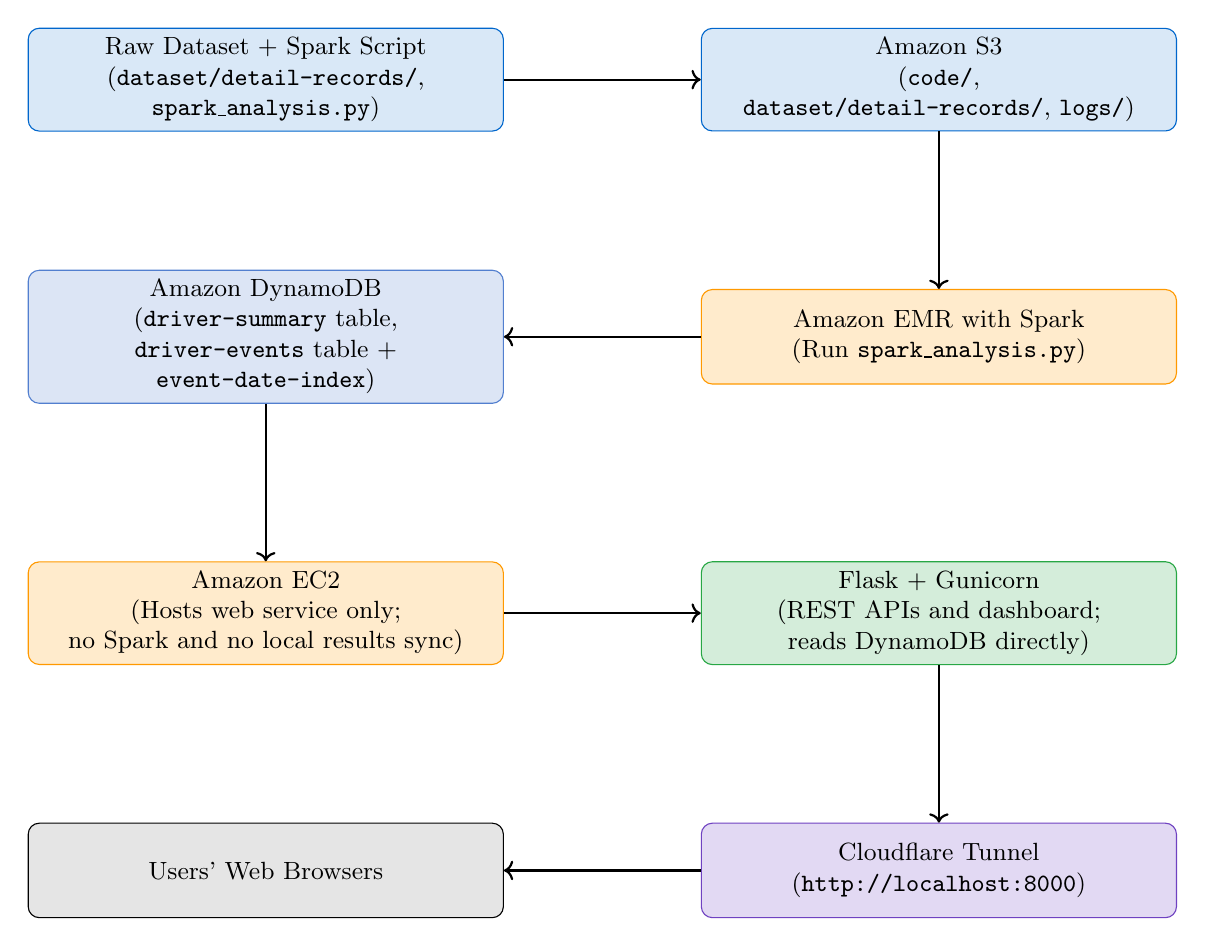
\begin{tikzpicture}[
    node distance=2.5cm,
    box/.style={
        rectangle,
        rounded corners,
        draw=black,
        align=center,
        minimum height=1.2cm,
        text width=5.8cm,
        font=\small
    },
    arrow/.style={->, thick}
]

% Colors
\definecolor{s3blue}{RGB}{0,102,204}
\definecolor{emrorange}{RGB}{255,153,0}
\definecolor{ddbblue}{RGB}{82,127,207}
\definecolor{ec2orange}{RGB}{255,153,0}
\definecolor{appgreen}{RGB}{40,167,69}
\definecolor{netpurple}{RGB}{111,66,193}

% Row 1
\node[box, fill=s3blue!15, draw=s3blue] (a) {
Raw Dataset + Spark Script\\
(\texttt{dataset/detail-records/}, \texttt{spark\_analysis.py})
};

\node[box, right=of a, fill=s3blue!15, draw=s3blue] (b) {
Amazon S3\\
(\texttt{code/}, \texttt{dataset/detail-records/}, \texttt{logs/})
};

% Row 2
\node[box, below=2cm of b, fill=emrorange!20, draw=emrorange] (c) {
Amazon EMR with Spark\\
(Run \texttt{spark\_analysis.py})
};

\node[box, left=of c, fill=ddbblue!20, draw=ddbblue] (d) {
Amazon DynamoDB\\
(\texttt{driver-summary} table,\\
\texttt{driver-events} table +\\
\texttt{event-date-index})
};

% Row 3
\node[box, below=2cm of d, fill=ec2orange!20, draw=ec2orange] (e) {
Amazon EC2\\
(Hosts web service only;\\
no Spark and no local results sync)
};

\node[box, right=of e, fill=appgreen!20, draw=appgreen] (f) {
Flask + Gunicorn\\
(REST APIs and dashboard;\\
reads DynamoDB directly)
};

% Row 4
\node[box, below=2cm of f, fill=netpurple!20, draw=netpurple] (g) {
Cloudflare Tunnel\\
(\texttt{http://localhost:8000})
};

\node[box, left=of g, fill=gray!20] (h) {
Users' Web Browsers
};

% Arrows
\draw[arrow] (a) -- (b);

\draw[arrow] (b) -- ++(0,-1) -- (c);

\draw[arrow] (c) -- (d);

\draw[arrow] (d) -- ++(0,-1) -- (e);

\draw[arrow] (e) -- (f);

\draw[arrow] (f) -- ++(0,-1) -- (g);

\draw[arrow] (g) -- (h);

\end{tikzpicture}


This design meets the project criteria for using AWS and Spark. It also showcases an integration of various cloud services for a distributed storage solution: S3 acts as storage, EMR as a data processing framework, EC2 for web server hosting, and Cloudflare Tunnel to enable a secure and public connection to the application.

% =========================
\section{Driver Behavior Summary Calculation}

The driver behavior summary is generated by the Spark data processing module. The raw driving records are grouped by \texttt{driverID} and \texttt{carPlateNumber}. After grouping, the system calculates the total number of each driving behavior for every driver.

The following metrics are calculated for each driver:

\begin{itemize}
    \item \textbf{Overspeed Count}: total number of overspeed records
    \item \textbf{Overspeed Time}: total duration of overspeed behavior in seconds
    \item \textbf{Fatigue Count}: total number of fatigue driving records
    \item \textbf{Neutral Slide Count}: total number of neutral slide records
    \item \textbf{Neutral Slide Time}: total duration of neutral slide behavior in seconds
    \item \textbf{Rapid Speed-up Count}: total number of rapid speed-up records
    \item \textbf{Rapid Slowdown Count}: total number of rapid slowdown records
    \item \textbf{H-Throttle Stop Count}: total number of h-throttle stop records
    \item \textbf{Oil Leak Count}: total number of oil leak records
\end{itemize}

In addition to these basic statistics, the system also calculates a risk score for each driver. The raw risk score is calculated using a weighted formula:

\[
\begin{aligned}
\texttt{risk\_raw\_score} =
&\ 0.35 \times \texttt{overspeed\_count} \\
&+ 0.30 \times \texttt{fatigue\_count} \\
&+ 0.15 \times \texttt{neutral\_slide\_count} \\
&+ 0.10 \times \texttt{rapid\_speedup\_count} \\
&+ 0.10 \times \texttt{rapid\_slowdown\_count}
\end{aligned}
\]

The raw risk score is then normalized to a value between 0 and 100:

\[
\texttt{risk\_score}
=
\frac{
\texttt{risk\_raw\_score} - \min(\texttt{risk\_raw\_score})
}{
\max(\texttt{risk\_raw\_score}) - \min(\texttt{risk\_raw\_score})
}
\times 100
\]

Based on the normalized score, each driver is classified into one of three risk levels:

\begin{itemize}
    \item \textbf{High Risk}: \texttt{risk\_score} $\geq 70$
    \item \textbf{Medium Risk}: \texttt{risk\_score} $\geq 40$ and $< 70$
    \item \textbf{Low Risk}: \texttt{risk\_score} $< 40$
\end{itemize}

Finally, drivers are ranked by their \texttt{risk\_score} in descending order. This ranking is displayed in the summary table and the driver risk ranking panel on the website.


% =========================
% =========================
\section{Deployment Steps}

\subsection{Overview}

The production deployment uses \textbf{Amazon S3, Amazon EMR, Amazon DynamoDB, Amazon EC2, Gunicorn, systemd, and Cloudflare Tunnel}. The Spark analysis job is executed on Amazon EMR instead of directly on the web server. Amazon S3 stores the raw dataset, Spark script, EMR bootstrap script, and EMR logs. The processed analysis results are written directly to Amazon DynamoDB. The Amazon EC2 instance hosts the Flask web application and serves the dashboard with Gunicorn.

This architecture separates batch data processing from online web serving. EMR processes the raw driving records and writes the driver summary, behavior event records, and speed time-series data to DynamoDB. The EC2 web server does not run Spark and does not synchronize generated result files from S3. Instead, the Flask backend reads the processed data from DynamoDB and provides API endpoints for the frontend. Finally, Cloudflare Tunnel exposes the website publicly while keeping the Gunicorn service bound to \texttt{127.0.0.1:8000}.

The deployment flow is summarized as follows:

\begin{enumerate}
    \item Upload the Spark script and raw dataset to Amazon S3.
    \item Create the required Amazon DynamoDB tables for the processed results.
    \item Create an Amazon EMR cluster with Spark installed.
    \item Submit the PySpark analysis script as an EMR step.
    \item Write the processed driver summary, behavior event records, and speed time-series data to Amazon DynamoDB.
    \item Launch an Amazon EC2 instance for the Flask web application.
    \item Configure the Flask application to read processed data from DynamoDB.
    \item Serve the Flask application with Gunicorn and manage it with systemd.
    \item Expose the website through Cloudflare Tunnel.
\end{enumerate}

\subsection{Deployment Steps}

\subsubsection{Prepare S3 Storage}

\begin{itemize}
    \item Create an S3 bucket or a project prefix in an existing bucket.
    \item The project uses the following S3 layout:
\begin{lstlisting}
s3://PROJECT_BUCKET/project-harpy-eagle/code/
s3://PROJECT_BUCKET/project-harpy-eagle/bootstrap/
s3://PROJECT_BUCKET/project-harpy-eagle/dataset/detail-records/
s3://PROJECT_BUCKET/project-harpy-eagle/logs/
\end{lstlisting}

    \item The \texttt{code/} prefix stores the Spark analysis script.
    \item The \texttt{bootstrap/} prefix stores the EMR bootstrap script for installing \texttt{boto3}.
    \item The \texttt{dataset/detail-records/} prefix stores the raw driving behavior dataset.
    \item The \texttt{logs/} prefix stores EMR execution logs.
    \item The processed analysis results are not stored as JSON files in S3. They are written directly to Amazon DynamoDB.

    \item Upload the Spark script, bootstrap script, and raw dataset to S3:
\begin{lstlisting}
export AWS_REGION=ap-southeast-1

./scripts/upload_emr_assets_to_s3.sh \
s3://PROJECT_BUCKET/project-harpy-eagle
\end{lstlisting}

    \item If the local dataset is stored in a different directory, pass the dataset path explicitly:
\begin{lstlisting}
./scripts/upload_emr_assets_to_s3.sh \
s3://PROJECT_BUCKET/project-harpy-eagle \
/path/to/detail-records
\end{lstlisting}
\end{itemize}

\subsubsection{Prepare DynamoDB Tables}

\begin{itemize}
    \item Create the DynamoDB tables used by the Spark job and Flask backend:
\begin{lstlisting}
./scripts/create_dynamodb_tables.sh \
project-harpy-eagle-driver-summary \
project-harpy-eagle-driver-events
\end{lstlisting}

    \item The summary table stores per-driver summary records.
    \item The events table stores driver behavior events and speed time-series records.
    \item The events table also uses a global secondary index named \texttt{event-date-index} for date-based queries.
    \item The helper script uses on-demand billing, so no read or write capacity planning is needed for this project workload.
    \item Make sure the EMR EC2 instance profile can read and write the DynamoDB tables.
    \item Make sure the EC2 web server role can read the DynamoDB tables.
\end{itemize}

\subsubsection{Run Spark Analysis on Amazon EMR}

\begin{itemize}
    \item Create an Amazon EMR cluster with Spark installed.
    \item Configure the EMR log URI to the project S3 log prefix:
\begin{lstlisting}
s3://PROJECT_BUCKET/project-harpy-eagle/logs/
\end{lstlisting}

    \item Add the bootstrap action during EMR cluster creation:
\begin{lstlisting}
s3://PROJECT_BUCKET/project-harpy-eagle/bootstrap/install-boto3.sh
\end{lstlisting}

    \item This bootstrap script installs \texttt{boto3} on the EMR nodes, so the Spark job can write processed records to DynamoDB.
    \item Make sure the EMR EC2 instance profile has permission to:
    \begin{itemize}
        \item read the S3 \texttt{code/}, \texttt{bootstrap/}, and \texttt{dataset/detail-records/} prefixes,
        \item write to the S3 \texttt{logs/} prefix,
        \item read and write the DynamoDB summary and events tables.
    \end{itemize}

    \item Submit the Spark analysis as an EMR step:
\begin{lstlisting}
./deploy/emr/add_spark_step.sh \
j-XXXXXXXXXXXXX \
s3://PROJECT_BUCKET/project-harpy-eagle \
project-harpy-eagle-driver-summary \
project-harpy-eagle-driver-events
\end{lstlisting}

    \item The helper script submits a Spark job equivalent to:
\begin{lstlisting}
spark-submit --deploy-mode cluster \
s3://PROJECT_BUCKET/project-harpy-eagle/code/spark_analysis.py \
--input s3://PROJECT_BUCKET/project-harpy-eagle/dataset/detail-records/ \
--summary-table project-harpy-eagle-driver-summary \
--events-table project-harpy-eagle-driver-events \
--aws-region ap-southeast-1 \
--log-level ERROR
\end{lstlisting}

    \item The EMR step status can be checked with:
\begin{lstlisting}
aws emr describe-step \
--cluster-id <EMR_CLUSTER_ID> \
--step-id <EMR_STEP_ID> \
--region ap-southeast-1
\end{lstlisting}

    \item A successful execution should show the step state as \texttt{COMPLETED}.
    \item After the EMR step completes, verify that DynamoDB contains the processed records:
\begin{lstlisting}
aws dynamodb scan \
--table-name project-harpy-eagle-driver-summary \
--select COUNT \
--region ap-southeast-1

aws dynamodb scan \
--table-name project-harpy-eagle-driver-events \
--select COUNT \
--region ap-southeast-1
\end{lstlisting}
\end{itemize}

\subsubsection{EC2 Web Server Setup}

\begin{itemize}
    \item Launch an Ubuntu 24.04 EC2 instance for the web application.
    \item Attach an IAM role to the EC2 instance so that it can read the DynamoDB tables.
    \item Since the backend is exposed through Cloudflare Tunnel, it is not necessary to open port \texttt{8000} publicly.
    \item SSH access on port \texttt{22} is required for deployment and maintenance.
    \item The EC2 web server does not need to run Spark, Java, or PySpark. It only serves the Flask application and reads processed data from DynamoDB.

    \item Connect to the EC2 instance:
\begin{lstlisting}
ssh -i /path/to/key.pem ubuntu@<EC2_PUBLIC_IP>
\end{lstlisting}

    \item Install required system packages:
\begin{lstlisting}
sudo apt update
sudo apt install -y git python3 python3-venv python3-pip unzip curl
\end{lstlisting}

    \item Clone the project repository under \texttt{/opt}:
\begin{lstlisting}
cd /opt
sudo git clone https://github.com/FivespeedDoc/project-harpy-eagle.git
sudo chown -R ubuntu:www-data /opt/project-harpy-eagle
cd /opt/project-harpy-eagle
\end{lstlisting}

    \item Create a Python virtual environment and install backend dependencies:
\begin{lstlisting}
python3 -m venv .venv
source .venv/bin/activate
python -m pip install --upgrade pip
pip install -r requirements.txt
\end{lstlisting}

    \item Create the production environment file:
\begin{lstlisting}
sudo cp .env.example /etc/project-harpy-eagle.env
sudo chown root:root /etc/project-harpy-eagle.env
sudo chmod 644 /etc/project-harpy-eagle.env
sudo nano /etc/project-harpy-eagle.env
\end{lstlisting}

    \item The main environment variables are:
\begin{lstlisting}
AWS_REGION=ap-southeast-1
DDB_SUMMARY_TABLE=project-harpy-eagle-driver-summary
DDB_EVENTS_TABLE=project-harpy-eagle-driver-events
DDB_EVENTS_DATE_INDEX=event-date-index
GUNICORN_BIND=127.0.0.1:8000
GUNICORN_WORKERS=2
GUNICORN_THREADS=4
GUNICORN_TIMEOUT=120
\end{lstlisting}
\end{itemize}

\subsubsection{Backend Setup}

\begin{itemize}
    \item First, smoke-test the Flask development server:
\begin{lstlisting}
cd /opt/project-harpy-eagle
source .venv/bin/activate
set -a
source /etc/project-harpy-eagle.env
set +a
python app.py
\end{lstlisting}

    \item In another shell, verify the health endpoints:
\begin{lstlisting}
curl http://127.0.0.1:5000/health
curl http://127.0.0.1:5000/ready
\end{lstlisting}

    \item Then test the production Gunicorn server:
\begin{lstlisting}
cd /opt/project-harpy-eagle
source .venv/bin/activate
set -a
source /etc/project-harpy-eagle.env
set +a
gunicorn --config deploy/gunicorn.conf.py wsgi:app
\end{lstlisting}

    \item If Gunicorn starts correctly, it should be reachable locally:
\begin{lstlisting}
curl http://127.0.0.1:8000
curl http://127.0.0.1:8000/health
curl http://127.0.0.1:8000/ready
\end{lstlisting}

    \item The \texttt{/health} endpoint reports whether the backend process is alive and shows the configured data backend.
    \item The \texttt{/ready} endpoint returns success only when the DynamoDB tables are accessible and populated.
\end{itemize}

\subsubsection{System Service Configuration}

\begin{itemize}
    \item To ensure that the backend starts automatically and restarts after failures, install the systemd service file:
\begin{lstlisting}
sudo cp deploy/systemd/project-harpy-eagle.service \
/etc/systemd/system/
\end{lstlisting}

    \item The current service file uses:
\begin{lstlisting}
WorkingDirectory=/opt/project-harpy-eagle
EnvironmentFile=/etc/project-harpy-eagle.env
ExecStart=/opt/project-harpy-eagle/.venv/bin/gunicorn --config /opt/project-harpy-eagle/deploy/gunicorn.conf.py wsgi:app
\end{lstlisting}

    \item If the project path or Linux username is different, edit the service file before starting it.
    \item Reload systemd, enable the service, and start it:
\begin{lstlisting}
sudo systemctl daemon-reload
sudo systemctl enable project-harpy-eagle
sudo systemctl start project-harpy-eagle
sudo systemctl status project-harpy-eagle
\end{lstlisting}

    \item For troubleshooting, inspect the backend service logs:
\begin{lstlisting}
sudo journalctl -u project-harpy-eagle -n 100 --no-pager
sudo journalctl -u project-harpy-eagle -f
\end{lstlisting}
\end{itemize}

\subsubsection{Cloudflare Tunnel}

\begin{itemize}
    \item Cloudflare Tunnel was used to expose the website securely without opening the Gunicorn port directly to the public Internet.
    \item Gunicorn listens locally on \texttt{127.0.0.1:8000}.
    \item Cloudflare Tunnel forwards external HTTPS requests to the local Gunicorn service.

    \item Install \texttt{cloudflared} on the EC2 instance:
\begin{lstlisting}
sudo mkdir -p --mode=0755 /usr/share/keyrings

curl -fsSL https://pkg.cloudflare.com/cloudflare-public-v2.gpg | \
sudo tee /usr/share/keyrings/cloudflare-public-v2.gpg >/dev/null

echo "deb [signed-by=/usr/share/keyrings/cloudflare-public-v2.gpg] https://pkg.cloudflare.com/cloudflared any main" | \
sudo tee /etc/apt/sources.list.d/cloudflared.list

sudo apt-get update
sudo apt-get install -y cloudflared
\end{lstlisting}

    \item Create a tunnel in the Cloudflare Zero Trust dashboard.
    \item Configure a public hostname and map it to the local backend service:
\begin{lstlisting}
http://localhost:8000
\end{lstlisting}

    \item Install and start the tunnel connector on the EC2 instance using the token generated by Cloudflare:
\begin{lstlisting}
sudo cloudflared service install <TUNNEL_TOKEN>
sudo systemctl enable cloudflared
sudo systemctl start cloudflared
sudo systemctl status cloudflared
\end{lstlisting}

    \item With this setup, external users access the public domain name, Cloudflare receives the request, and the request is forwarded through the tunnel to the Gunicorn service running on the EC2 instance.
\end{itemize}

\subsection{Update Procedure}

\subsubsection{Updating the Dataset and Analysis Results}

\begin{enumerate}
    \item Upload the new dataset files to the S3 dataset prefix:
\begin{lstlisting}
aws s3 sync ./detail-records/ \
s3://PROJECT_BUCKET/project-harpy-eagle/dataset/detail-records/ \
--region ap-southeast-1
\end{lstlisting}

    \item Submit the EMR Spark analysis step again:
\begin{lstlisting}
./deploy/emr/add_spark_step.sh \
j-XXXXXXXXXXXXX \
s3://PROJECT_BUCKET/project-harpy-eagle \
project-harpy-eagle-driver-summary \
project-harpy-eagle-driver-events
\end{lstlisting}

    \item Wait until the EMR step state becomes \texttt{COMPLETED}.
    \item Verify that the DynamoDB tables contain the updated processed records:
\begin{lstlisting}
aws dynamodb scan \
--table-name project-harpy-eagle-driver-summary \
--select COUNT \
--region ap-southeast-1

aws dynamodb scan \
--table-name project-harpy-eagle-driver-events \
--select COUNT \
--region ap-southeast-1
\end{lstlisting}

    \item The Spark job normally performs idempotent upserts, so rerunning the same dataset updates matching records instead of creating duplicate event rows.
    \item The Flask backend does not need to synchronize result files from S3. It reads the latest processed data from DynamoDB.
    \item Restart the backend service only if the application configuration has changed:
\begin{lstlisting}
sudo systemctl restart project-harpy-eagle
sudo systemctl status project-harpy-eagle
\end{lstlisting}
\end{enumerate}

\subsubsection{Updating the Application Code}

\begin{enumerate}
    \item Connect to the EC2 instance and move to the project directory:
\begin{lstlisting}
ssh -i /path/to/key.pem ubuntu@<EC2_PUBLIC_IP>
cd /opt/project-harpy-eagle
\end{lstlisting}

    \item Pull the latest source code:
\begin{lstlisting}
git pull origin main
\end{lstlisting}

    \item Activate the virtual environment and update backend dependencies:
\begin{lstlisting}
source .venv/bin/activate
pip install -r requirements.txt
\end{lstlisting}

    \item If the Spark script or bootstrap script has changed, upload the updated EMR assets to S3 before submitting the next EMR step:
\begin{lstlisting}
./scripts/upload_emr_assets_to_s3.sh \
s3://PROJECT_BUCKET/project-harpy-eagle
\end{lstlisting}

    \item Restart the backend service:
\begin{lstlisting}
sudo systemctl restart project-harpy-eagle
sudo systemctl status project-harpy-eagle
\end{lstlisting}

    \item Cloudflare Tunnel does not need to be reconfigured if the local backend endpoint remains \texttt{http://localhost:8000}.
\end{enumerate}


\section{Design of Use Cases and Screenshots of Testing Results}

This section presents the functional testing design and testing results of the deployed driver behavior analysis website. The tests focus on whether the system satisfies the main project requirements: displaying driver behavior summaries, supporting period-based summary filtering, monitoring driver speed in near real time, showing overspeed warnings, and updating the speed visualization every 30 seconds.

\subsection{Testing Environment}

The functional tests were conducted on the deployed production website.

\begin{itemize}
    \item \textbf{Website URL:} \url{https://harpy-eagle.project-veracity.life}
    \item \textbf{Browser:} Apple Safari Version 26.2 (21623.1.14.11.9) on macOS Tahoe
    \item \textbf{Backend environment:} Flask application served by Gunicorn on Amazon EC2
    \item \textbf{Data processing environment:} PySpark job executed on Amazon EMR
    \item \textbf{Storage:} Amazon S3 for the raw dataset, Spark script, EMR bootstrap script, and EMR logs
    \item \textbf{Database:} Amazon DynamoDB for processed driver summary, behavior event records, and speed time-series data
    \item \textbf{Test dataset:} Driving behavior records of 10 drivers over 10 consecutive days
    \item \textbf{Testing method:} Manual functional testing and backend API smoke testing
\end{itemize}

\subsection{Use Case Design}

The following table summarizes the major functional test cases designed for the system.

\begin{small}
\setlength{\tabcolsep}{4pt}
\renewcommand{\arraystretch}{1.25}

\begin{longtable}{|p{1.2cm}|p{3.2cm}|p{5.0cm}|p{5.0cm}|p{1.5cm}|}
\caption{Test scenarios for our driver behavior analysis system}
\label{tab:functional-tests} \\
\hline
\textbf{ID} & \textbf{Function} & \textbf{Test Steps} & \textbf{Expected Result} & \textbf{Status} \\
\hline
\endfirsthead

\multicolumn{5}{c}%
{{\tablename\ \thetable{} -- continued from previous page}} \\
\hline
\textbf{ID} & \textbf{Function} & \textbf{Test Steps} & \textbf{Expected Result} & \textbf{Status} \\
\hline
\endhead

\hline
\multicolumn{5}{r}{{Continued on next page}} \\
\endfoot

\hline
\endlastfoot

FT-01 & Website loading & Open the deployed website URL in a browser. & The dashboard page loads successfully without runtime error. & Pass \\
\hline
FT-02 & Driver behavior summary & Open the \textit{Behavior Summary} tab. & The system displays the behavior summary table for all drivers. The table includes driver ID, car plate number, risk ranking, overspeed count, overspeed time, fatigue count, neutral slide count, and other behavior indicators. & Pass \\
\hline
FT-03 & Driver risk ranking & Check the risk ranking area and the risk columns in the summary table. & Drivers are ranked by normalized risk score and classified into high, medium, or low risk levels. & Pass \\
\hline
FT-04 & Period-based summary filtering & Select a start time and end time, then click \textit{Apply Period}. & The summary table is updated based on the selected time period. The period column also reflects the selected range. & Pass \\
\hline
FT-05 & Reset summary filter & Click the \textit{Reset} button after applying a period filter. & The summary table returns to the full-period result. & Pass \\
\hline
FT-06 & Driver list loading & Open the \textit{Speed Monitor} tab and check the driver selector. & The driver dropdown list is populated with available driver IDs from the backend API. & Pass \\
\hline
FT-07 & Single-driver speed monitoring & Select one driver and click \textit{Start Monitoring}. & The speed chart is displayed and speed records are loaded in batches. & Pass \\
\hline
FT-08 & Overspeed warning & Monitor a driver whose speed records contain overspeed records. & When speed exceeds the threshold, the website displays an overspeed warning message. & Pass \\
\hline
FT-09 & Driving trajectory map & Start monitoring a selected driver and inspect the map panel. & The driver's trajectory is displayed on the OpenStreetMap map, and the route follows the latitude and longitude records from the dataset. & Pass \\
\hline
FT-10 & 30-second automatic refresh & Start monitoring a driver and observe the chart update after 30 seconds. & The frontend automatically requests the next batch of speed records and updates the speed chart every 30 seconds. & Pass \\
\hline
FT-11 & Stop monitoring & Click the \textit{Stop} button during speed monitoring. & The monitoring process stops and the chart no longer fetches new batches automatically. & Pass \\
\hline
FT-12 & All-driver monitor & Open the \textit{All Drivers Monitor} tab. & The system displays speed curves for all drivers and updates them every 30 seconds. & Pass \\
\hline
FT-13 & Backend health check & Visit \texttt{/health} and \texttt{/ready}. & The backend returns the service status and indicates whether the DynamoDB-backed dashboard data is ready.
 & Pass \\
\hline
FT-14 & Invalid driver handling & Request speed data for a non-existing driver ID through \texttt{/api/speed/<driver\_id>}. & The backend returns an error response instead of crashing. & Pass \\
\hline

\end{longtable}
\end{small}


\subsection{Testing Results and Screenshots}

The following screenshots show the main testing results. The screenshots demonstrate that the website can load successfully, display driver behavior summaries, filter results by period, monitor speed data, show overspeed warnings, display driving trajectories, and check backend service status.

\subsubsection{Website Loading and Driver Behavior Summary}

Figure~\ref{fig:test-summary} shows that the deployed website can be opened successfully. The \textit{Behavior Summary} page displays the driver behavior table and risk ranking result.

\begin{figure}[H]
\centering
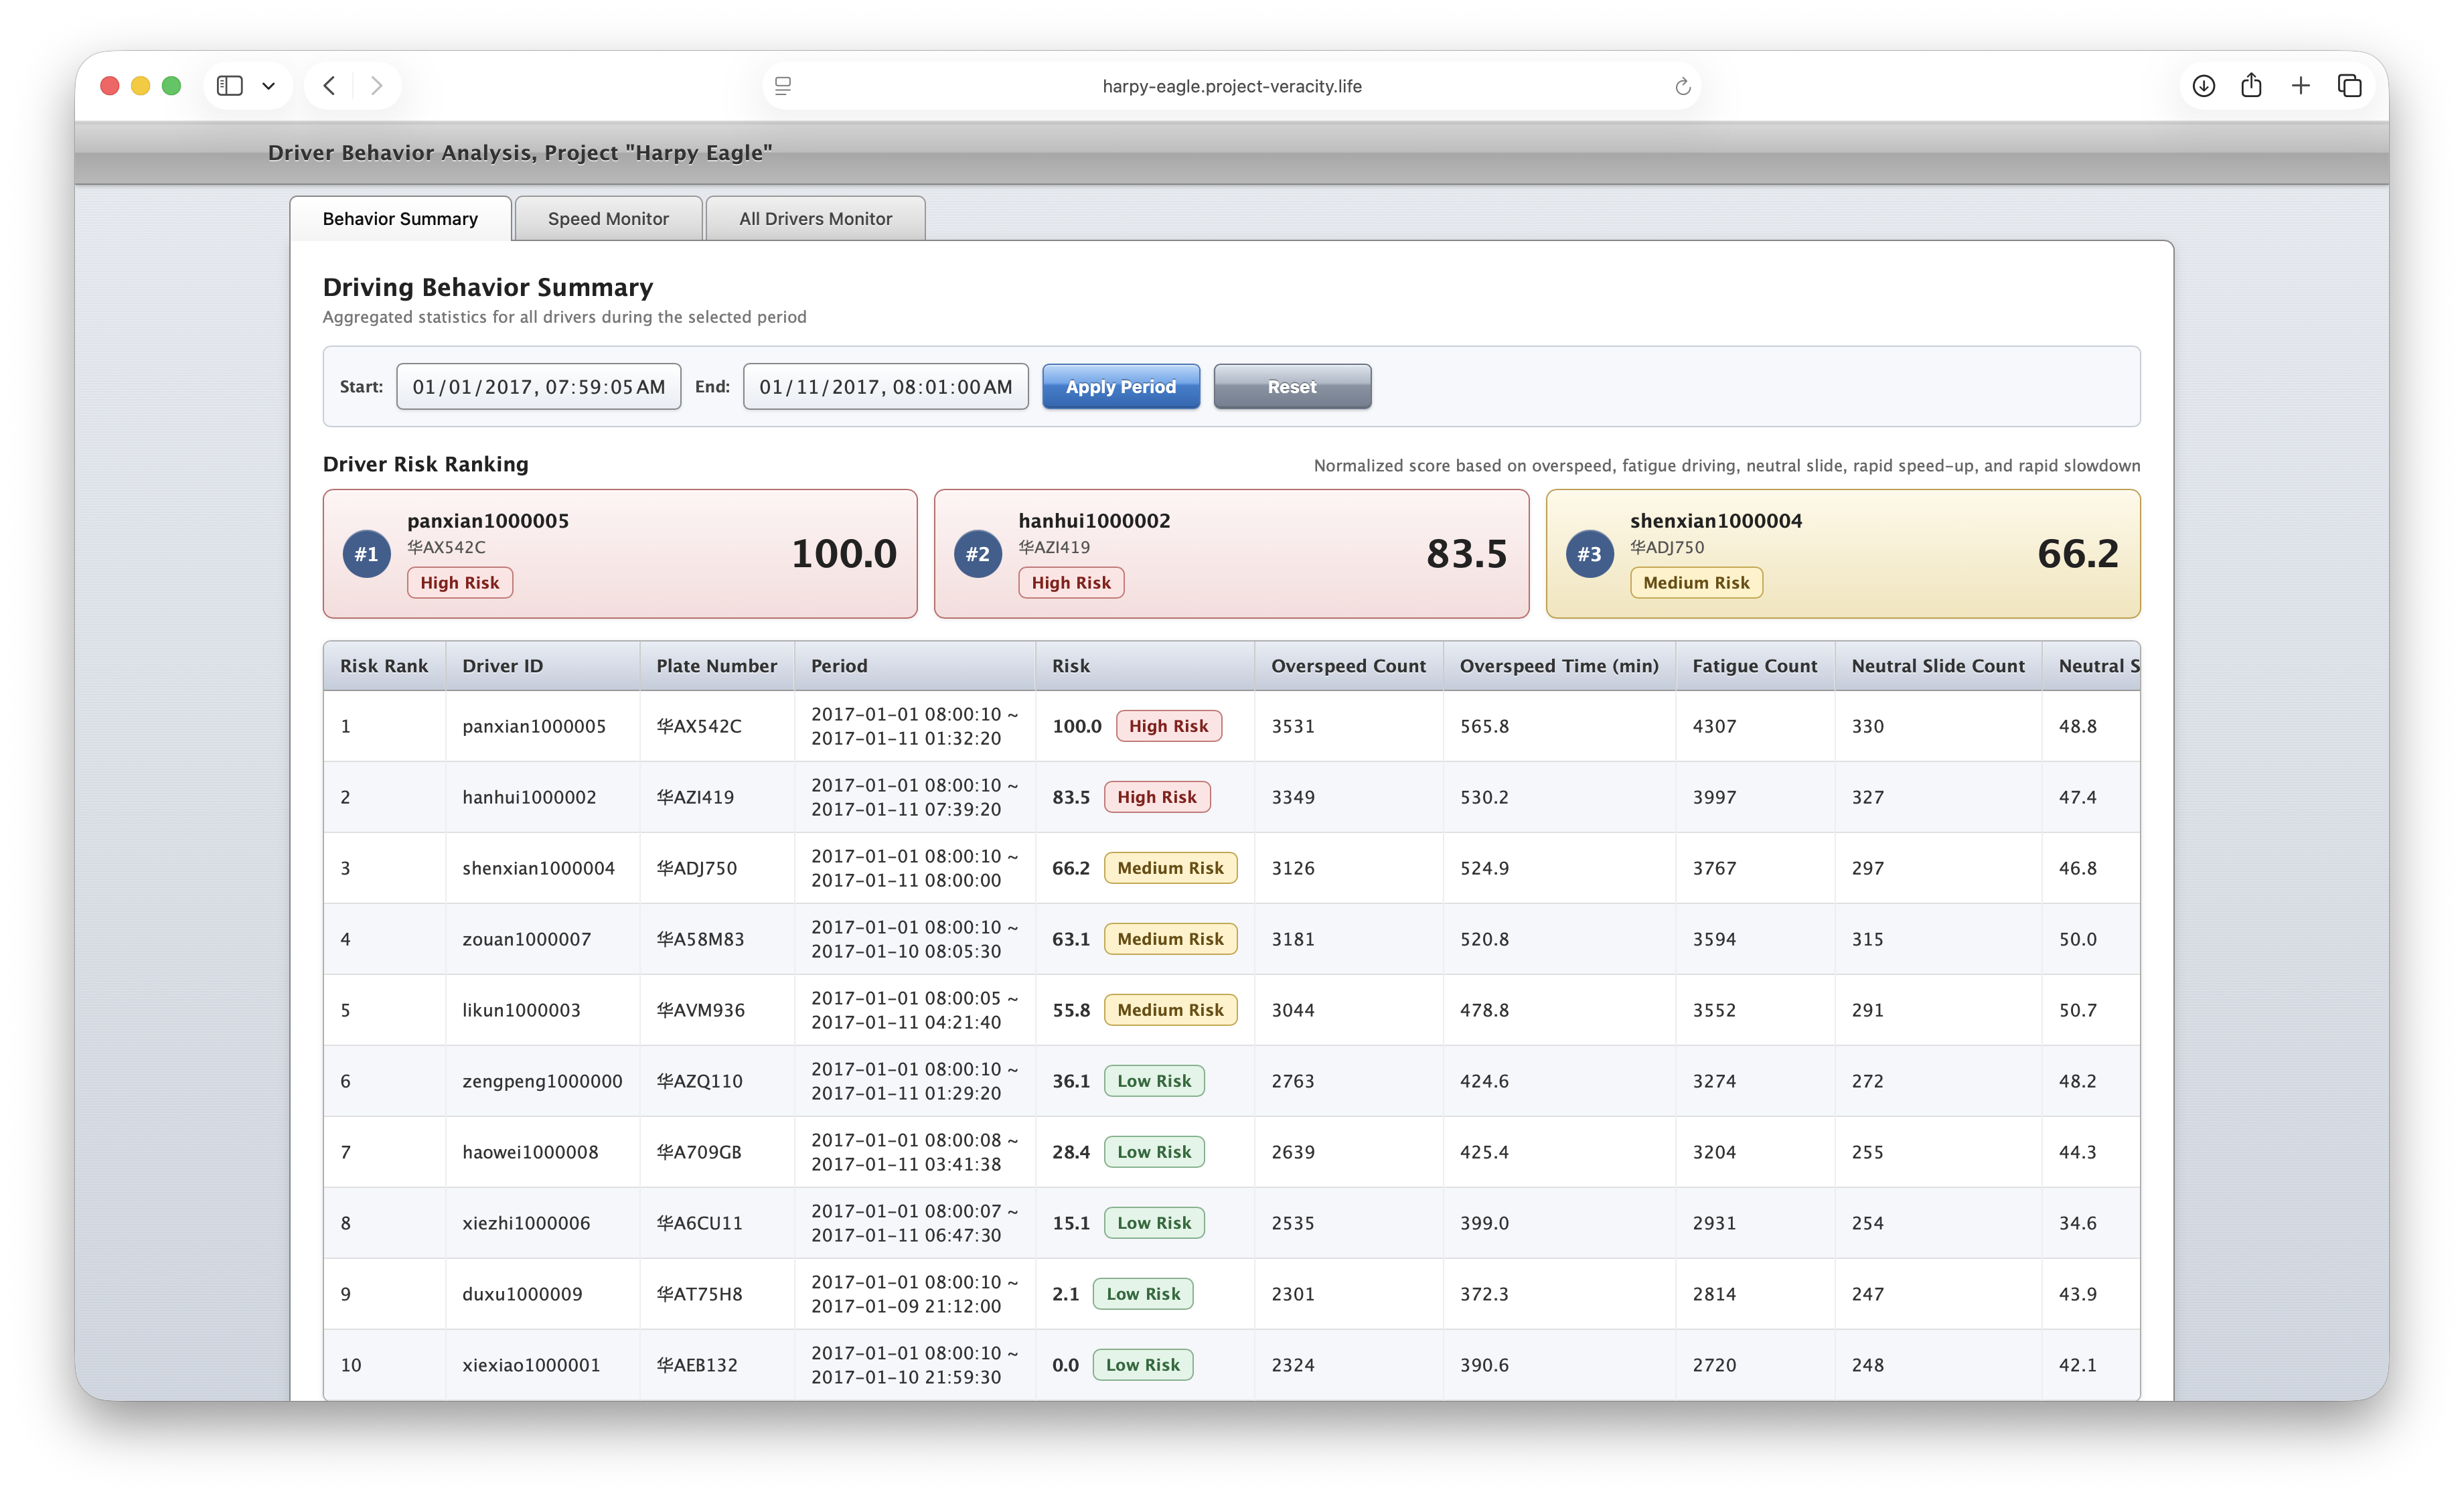
\includegraphics[width=0.9\textwidth]{test-summary.png}
\caption{Website loading and driver behavior summary test result}
\label{fig:test-summary}
\end{figure}

\subsubsection{Period-Based Summary Filtering}

Figure~\ref{fig:test-period-filter} shows the result after selecting a start time and end time. The table is updated according to the selected period, which verifies that the backend period aggregation API works correctly.

\begin{figure}[H]
\centering
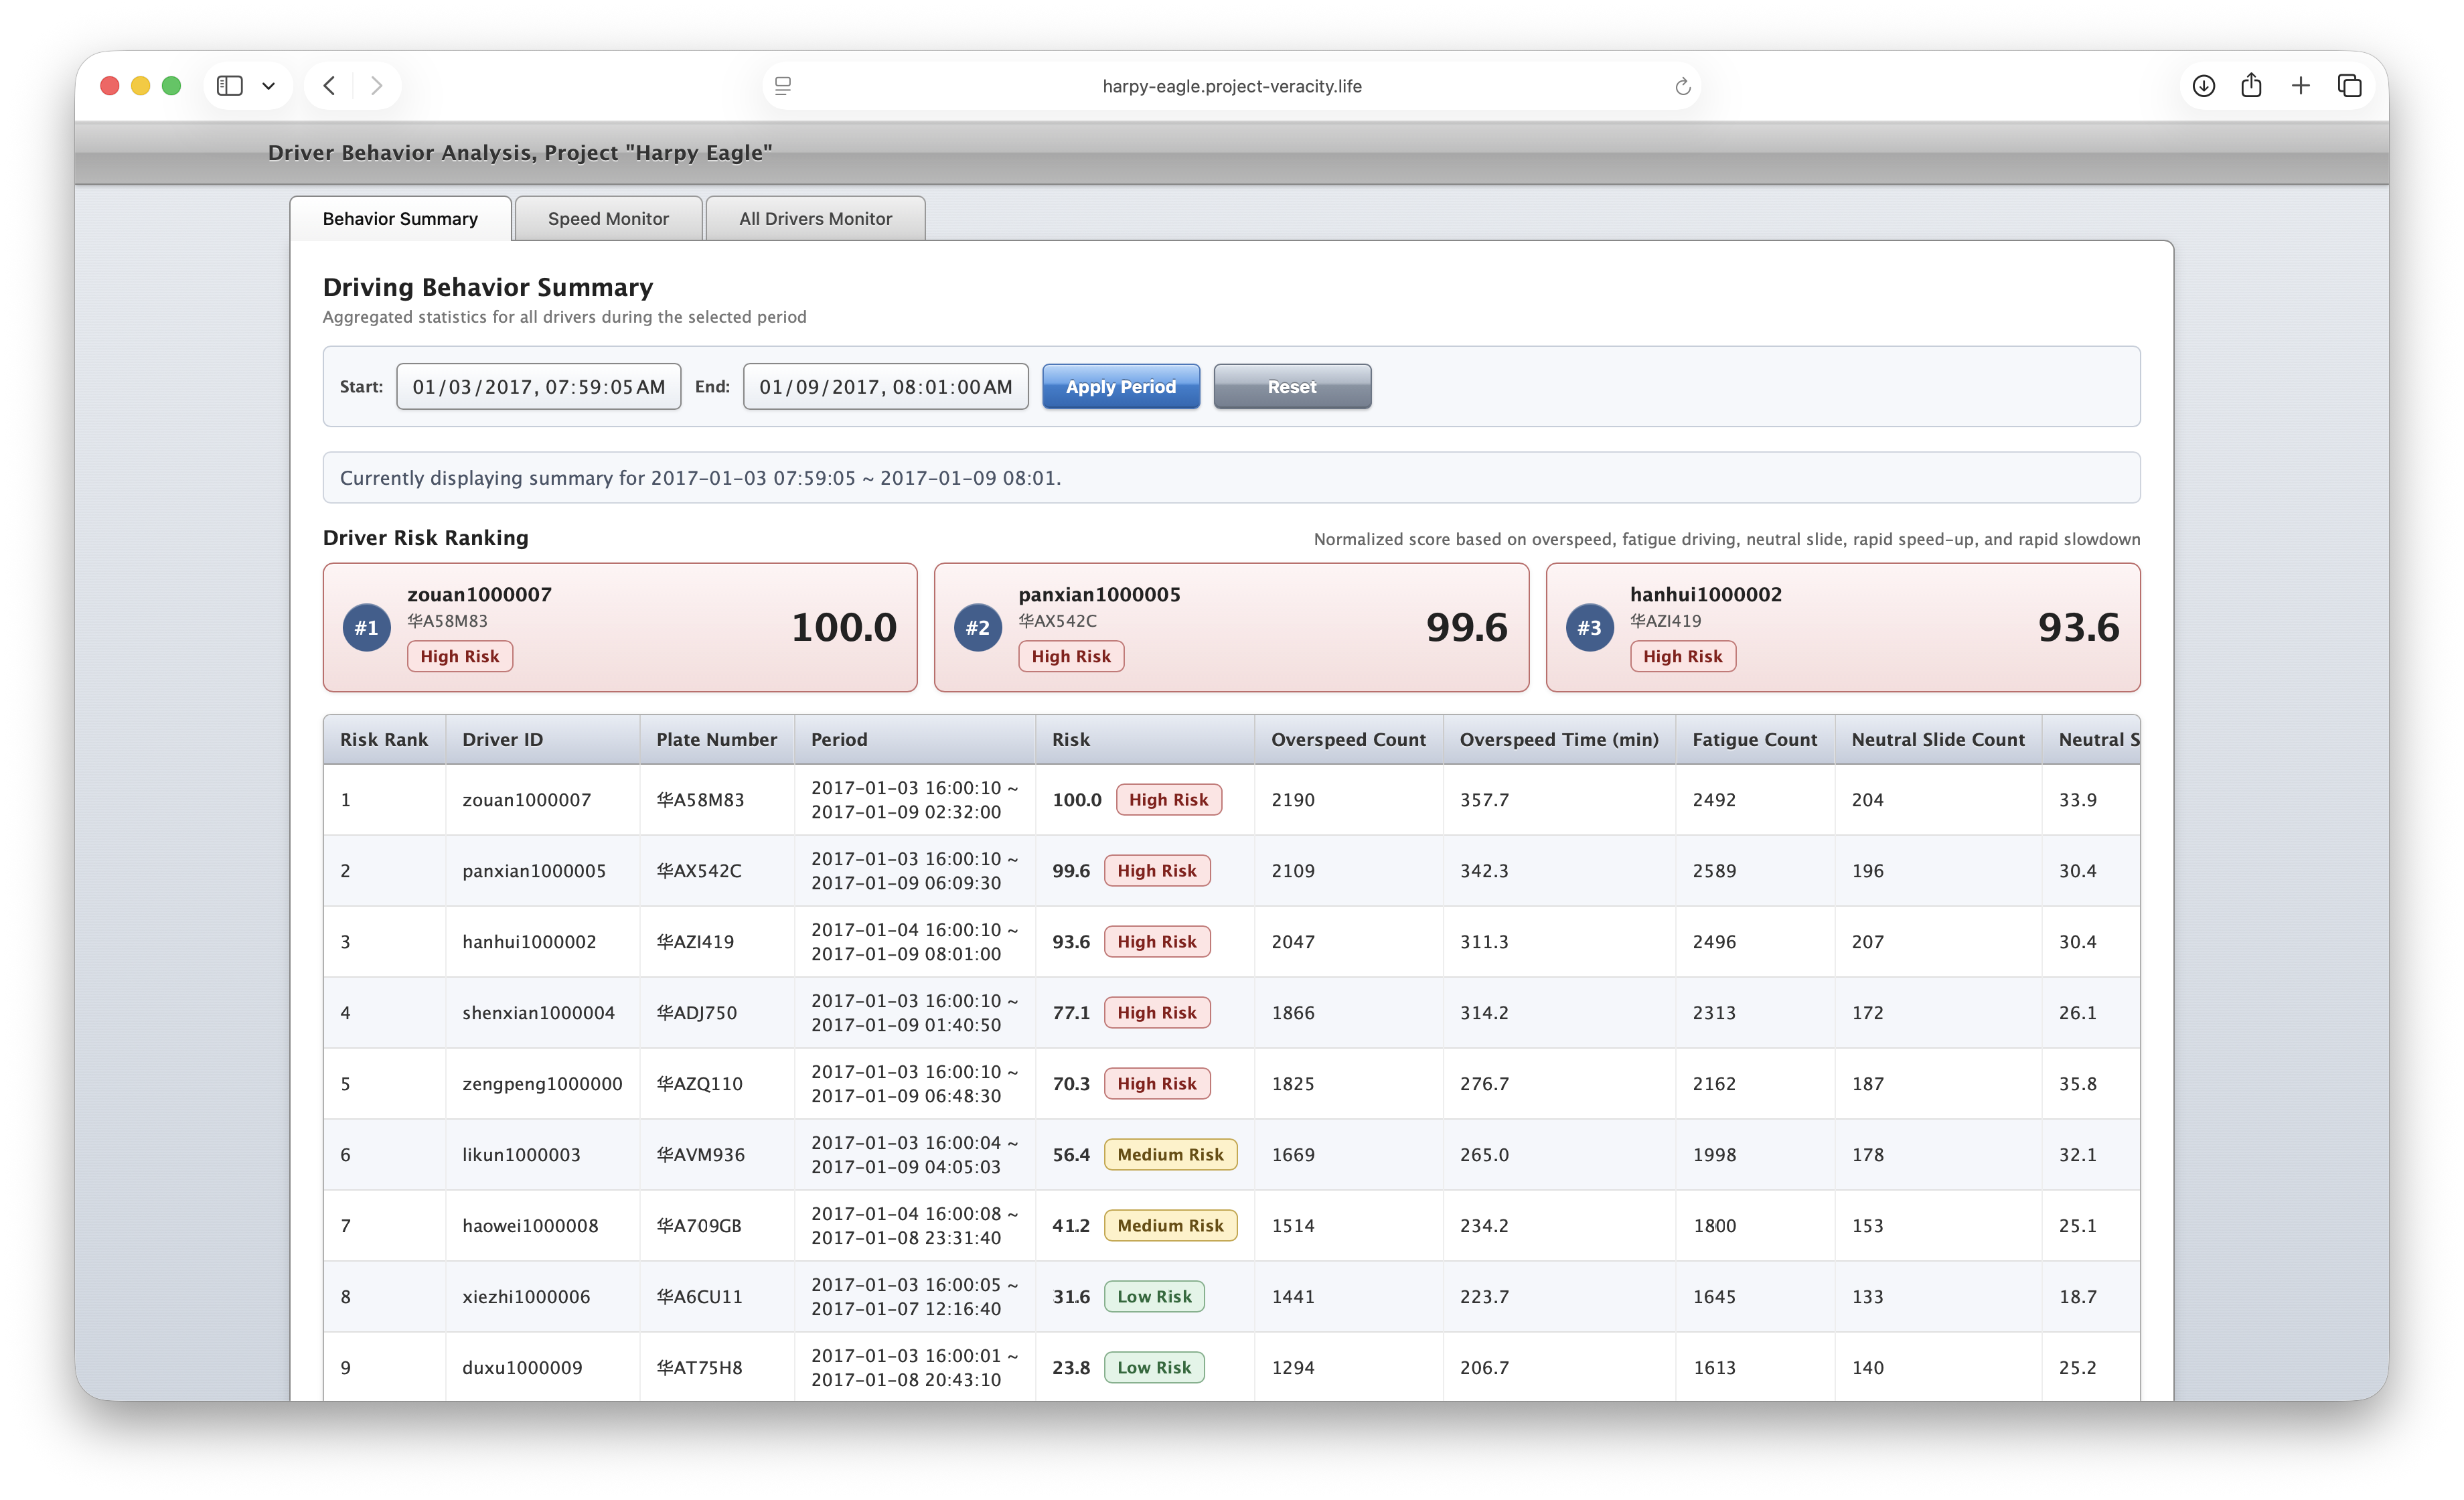
\includegraphics[width=0.9\textwidth]{test-period-filter.png}
\caption{Period-based behavior summary filtering test result}
\label{fig:test-period-filter}
\end{figure}

\subsubsection{Single-Driver Speed Monitoring}

Figure~\ref{fig:test-speed-monitor} shows the single-driver speed monitoring function. After a driver is selected and monitoring is started, the frontend loads speed records from the backend and visualizes them using a line chart.

\begin{figure}[H]
\centering
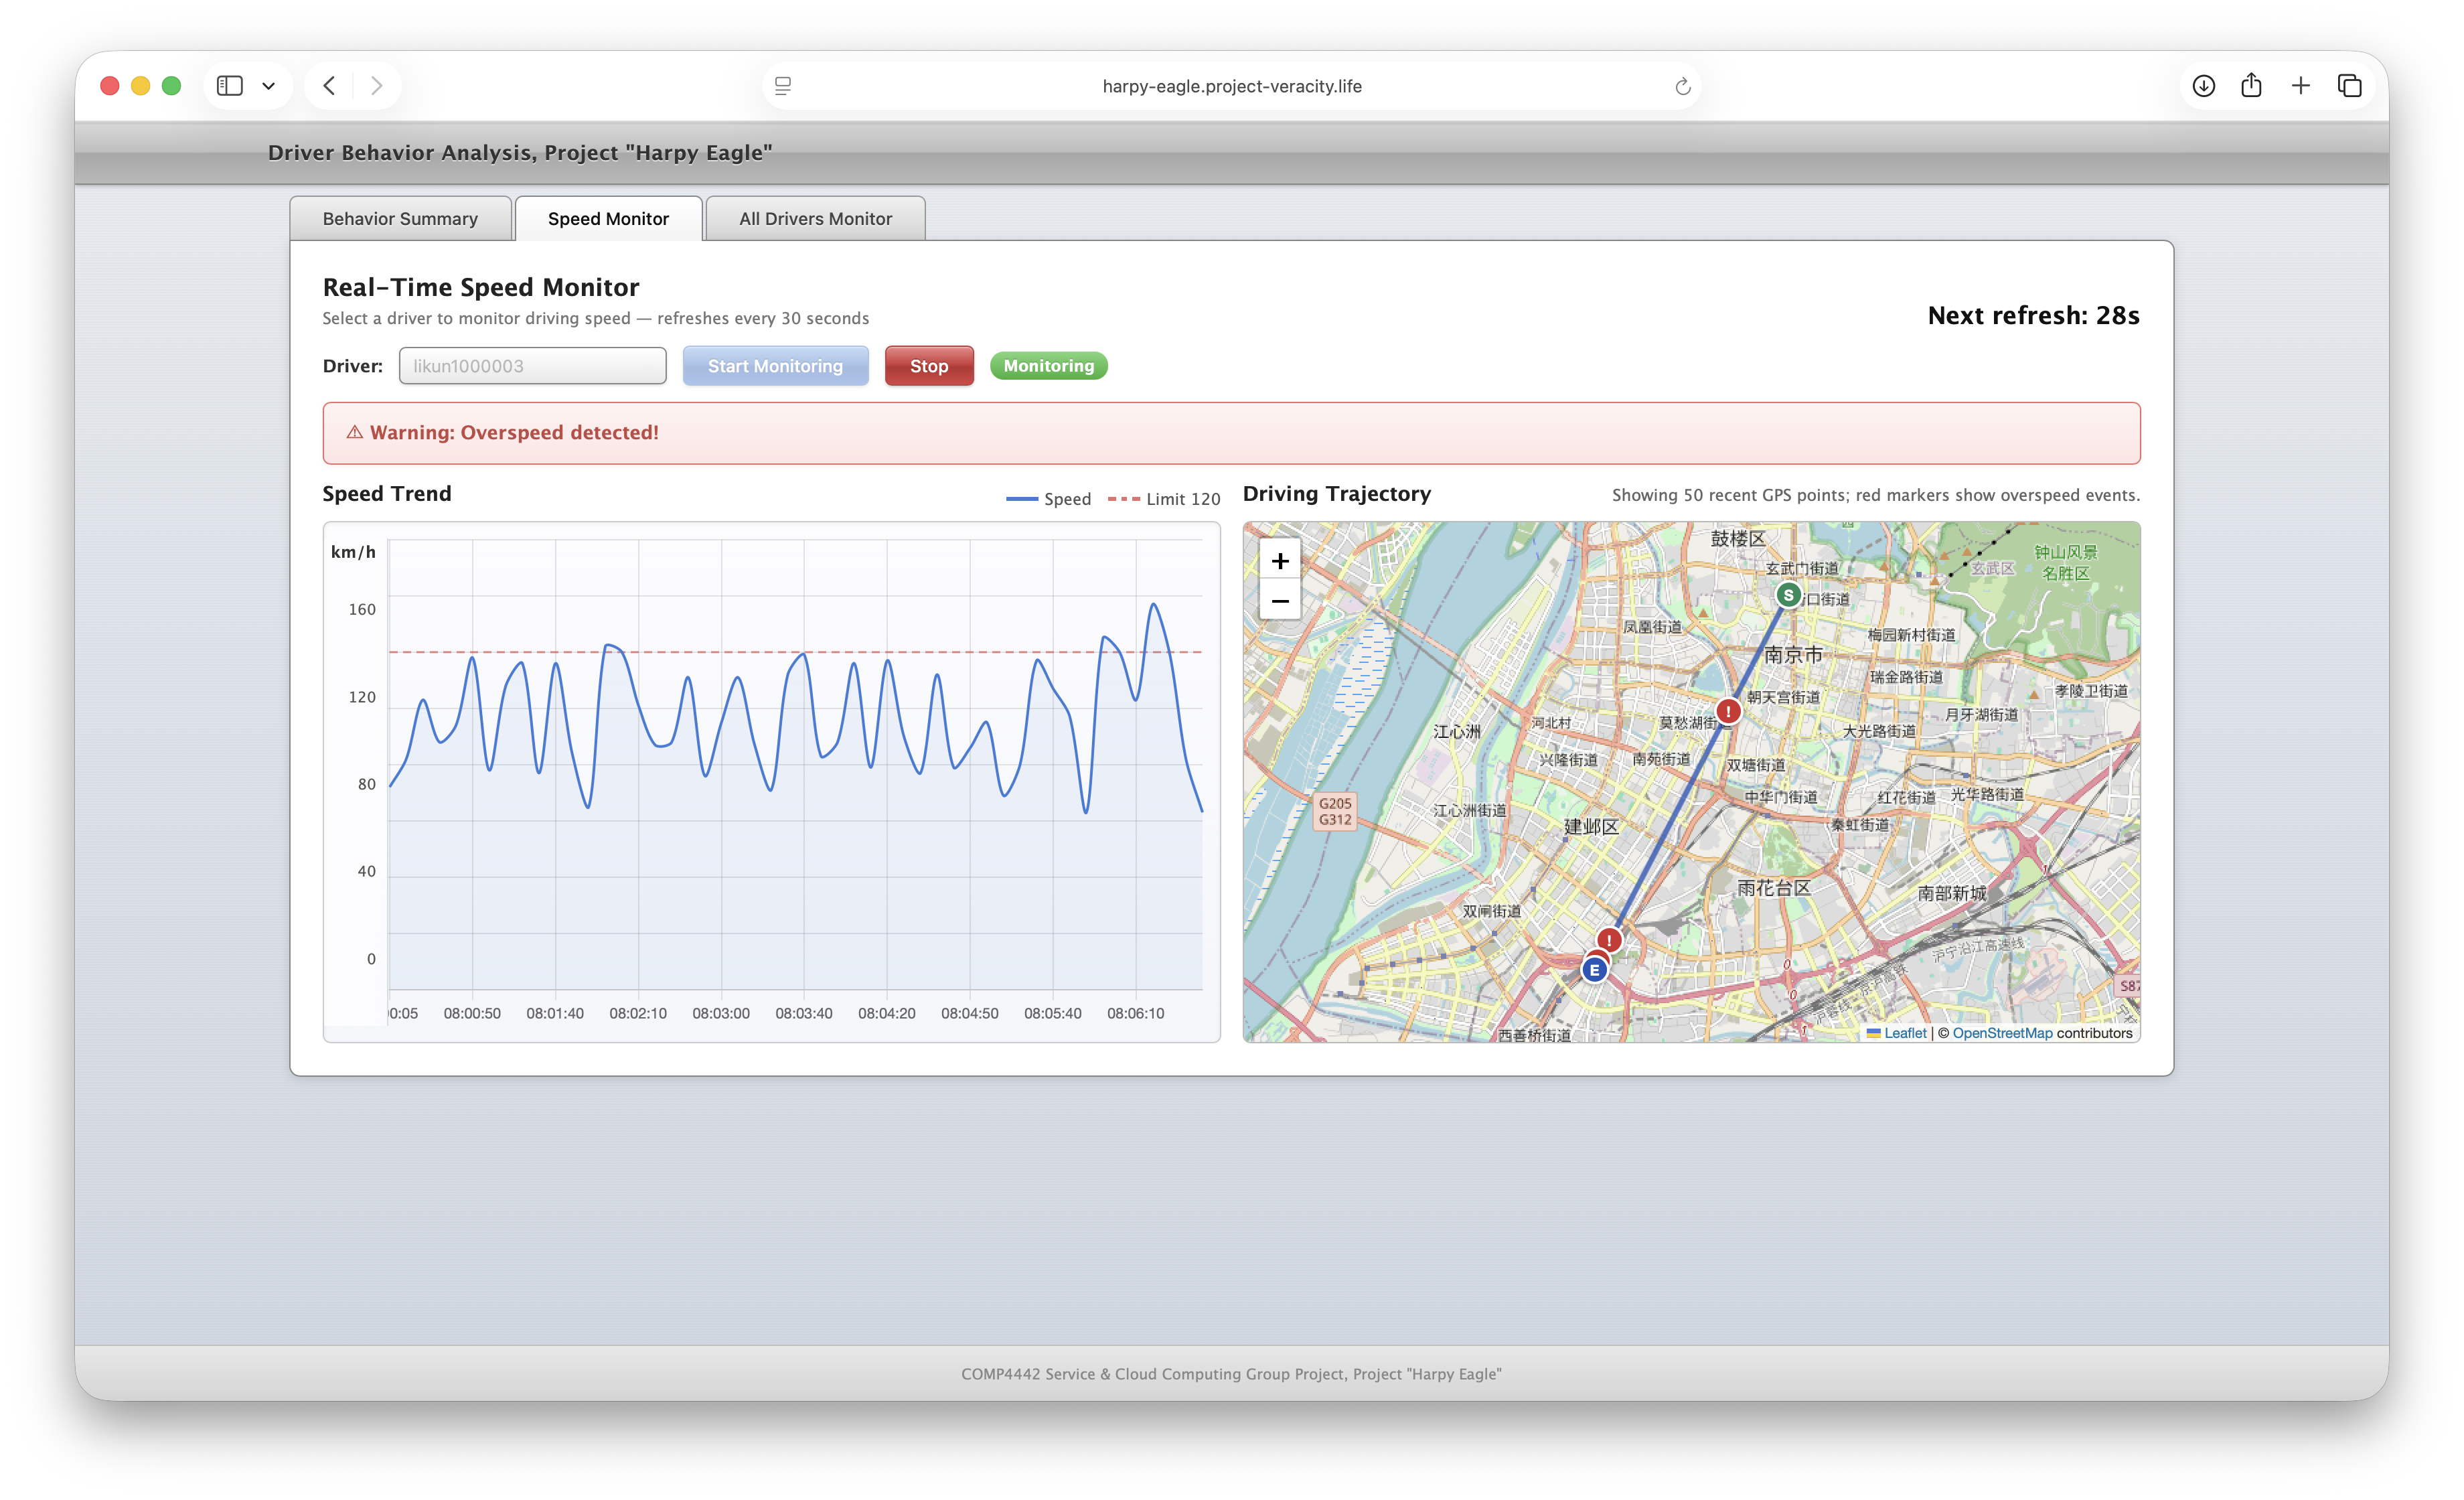
\includegraphics[width=0.9\textwidth]{test-speed-monitor.png}
\caption{Single-driver speed monitoring test result}
\label{fig:test-speed-monitor}
\end{figure}

\subsubsection{Overspeed Warning}

Figure~\ref{fig:test-overspeed-warning} shows that the system issues a warning when (at least one) overspeed records are detected. This verifies that the monitoring page can identify dangerous speed behavior and notify the user.

\begin{figure}[H]
\centering
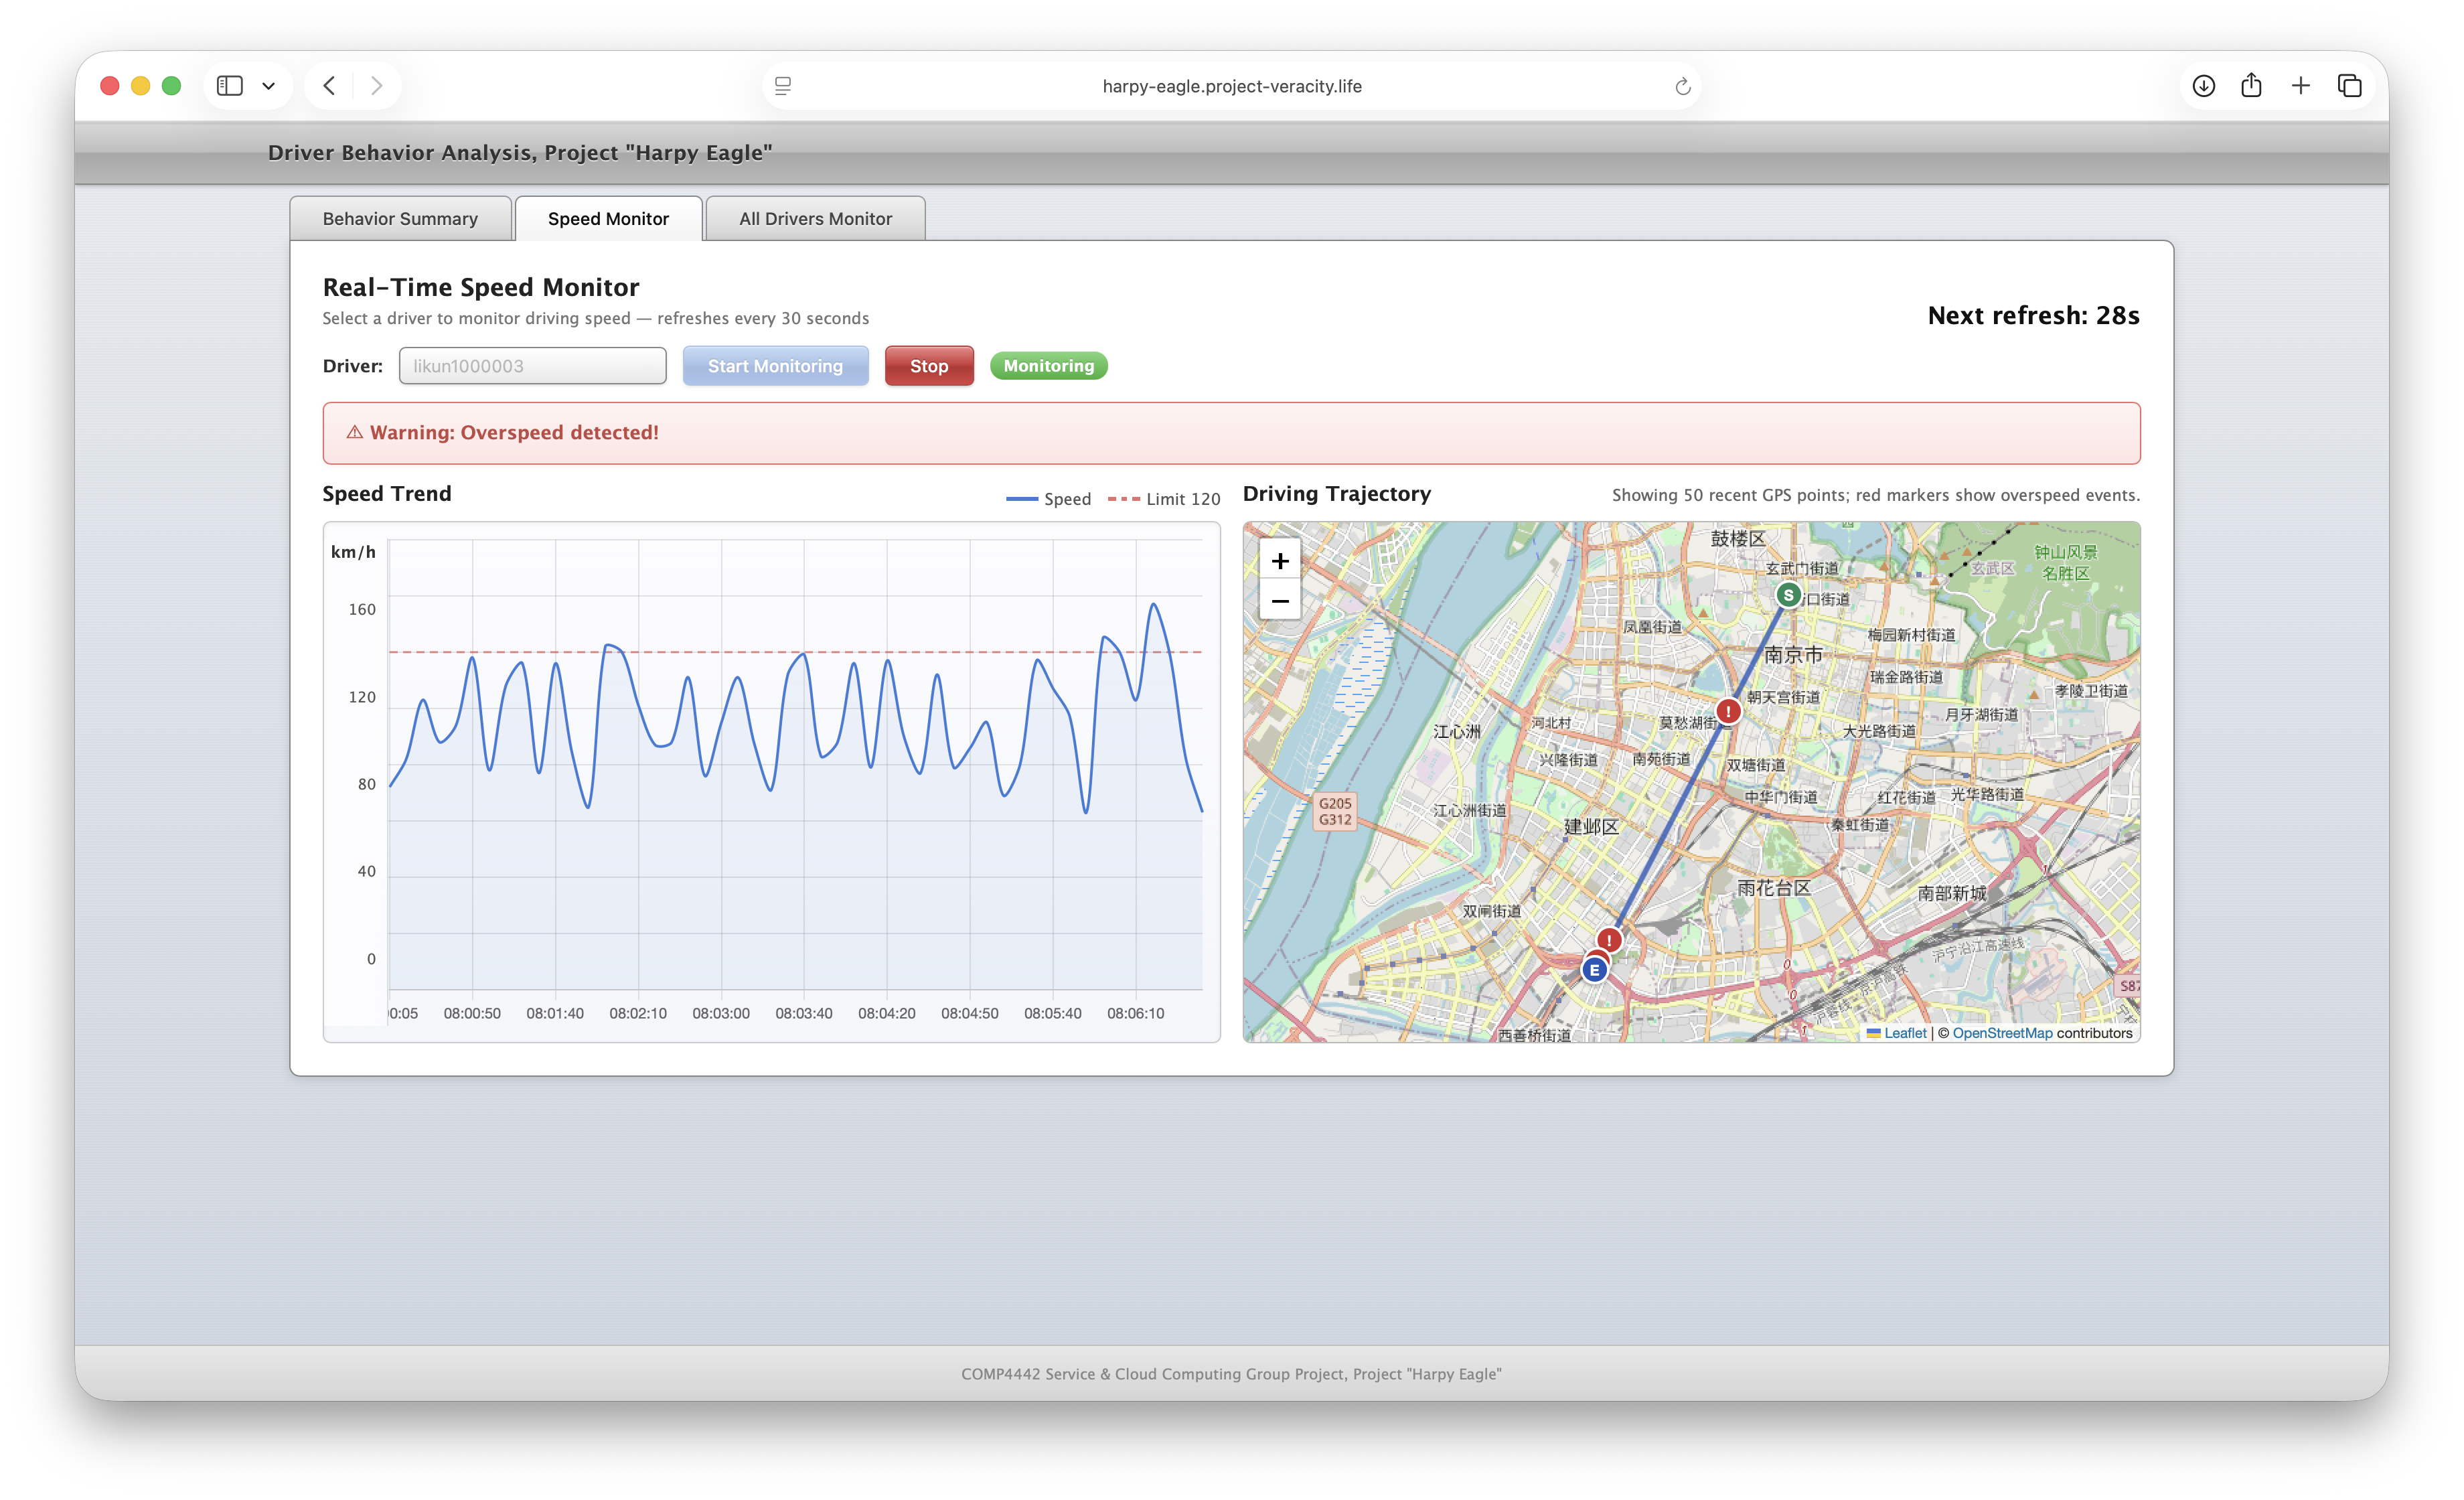
\includegraphics[width=0.9\textwidth]{test-speed-monitor.png}
\caption{Overspeed warning test result}
\label{fig:test-overspeed-warning}
\end{figure}

\subsubsection{Driving Trajectory Map}

Figure~\ref{fig:test-map} shows the driver's trajectory on the OpenStreetMap map. This verifies that the frontend correctly reads latitude and longitude records from the selected driver's speed data.

\begin{figure}[H]
\centering
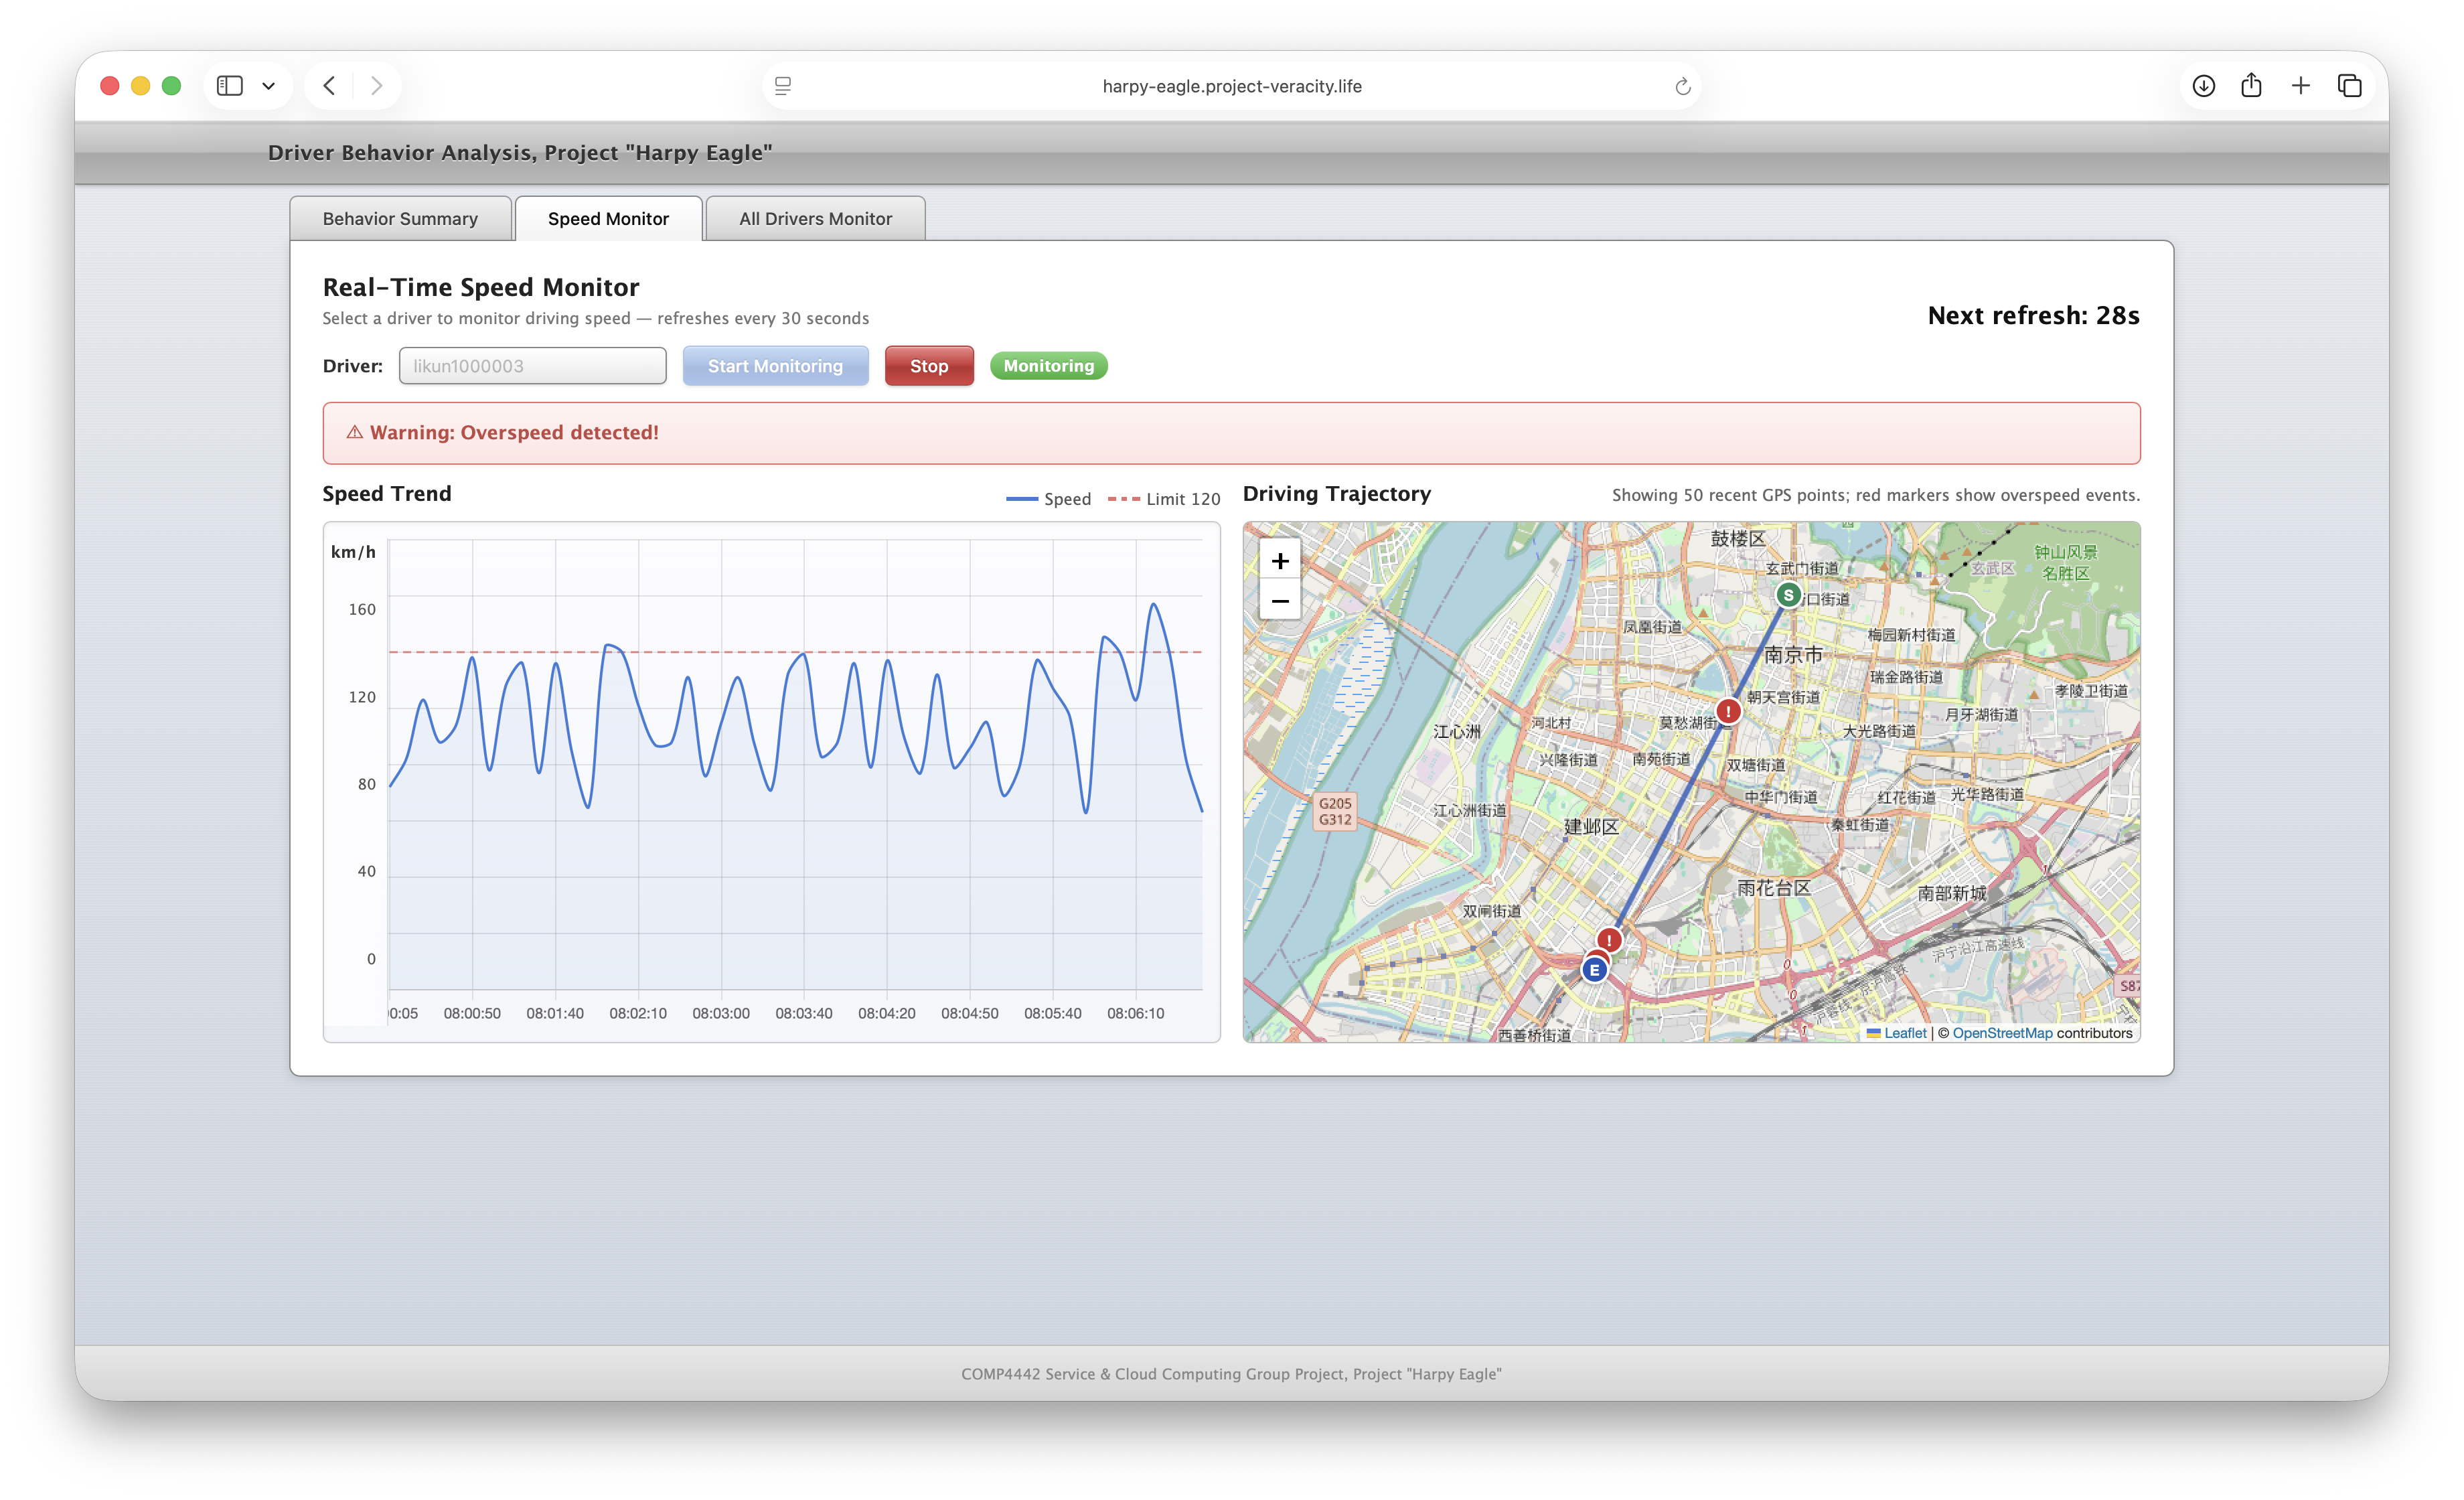
\includegraphics[width=0.9\textwidth]{test-speed-monitor.png}
\caption{Driving trajectory map test result}
\label{fig:test-map}
\end{figure}

\subsubsection{Automatic Refresh Every 30 Seconds}

Figure~\ref{fig:test-refresh-before} and Figure~\ref{fig:test-refresh-after} show the speed monitor before and after the 30-second refresh interval. The chart receives the next batch of speed records and updates automatically, which verifies the near real-time monitoring behavior.

\begin{figure}[H]
\centering
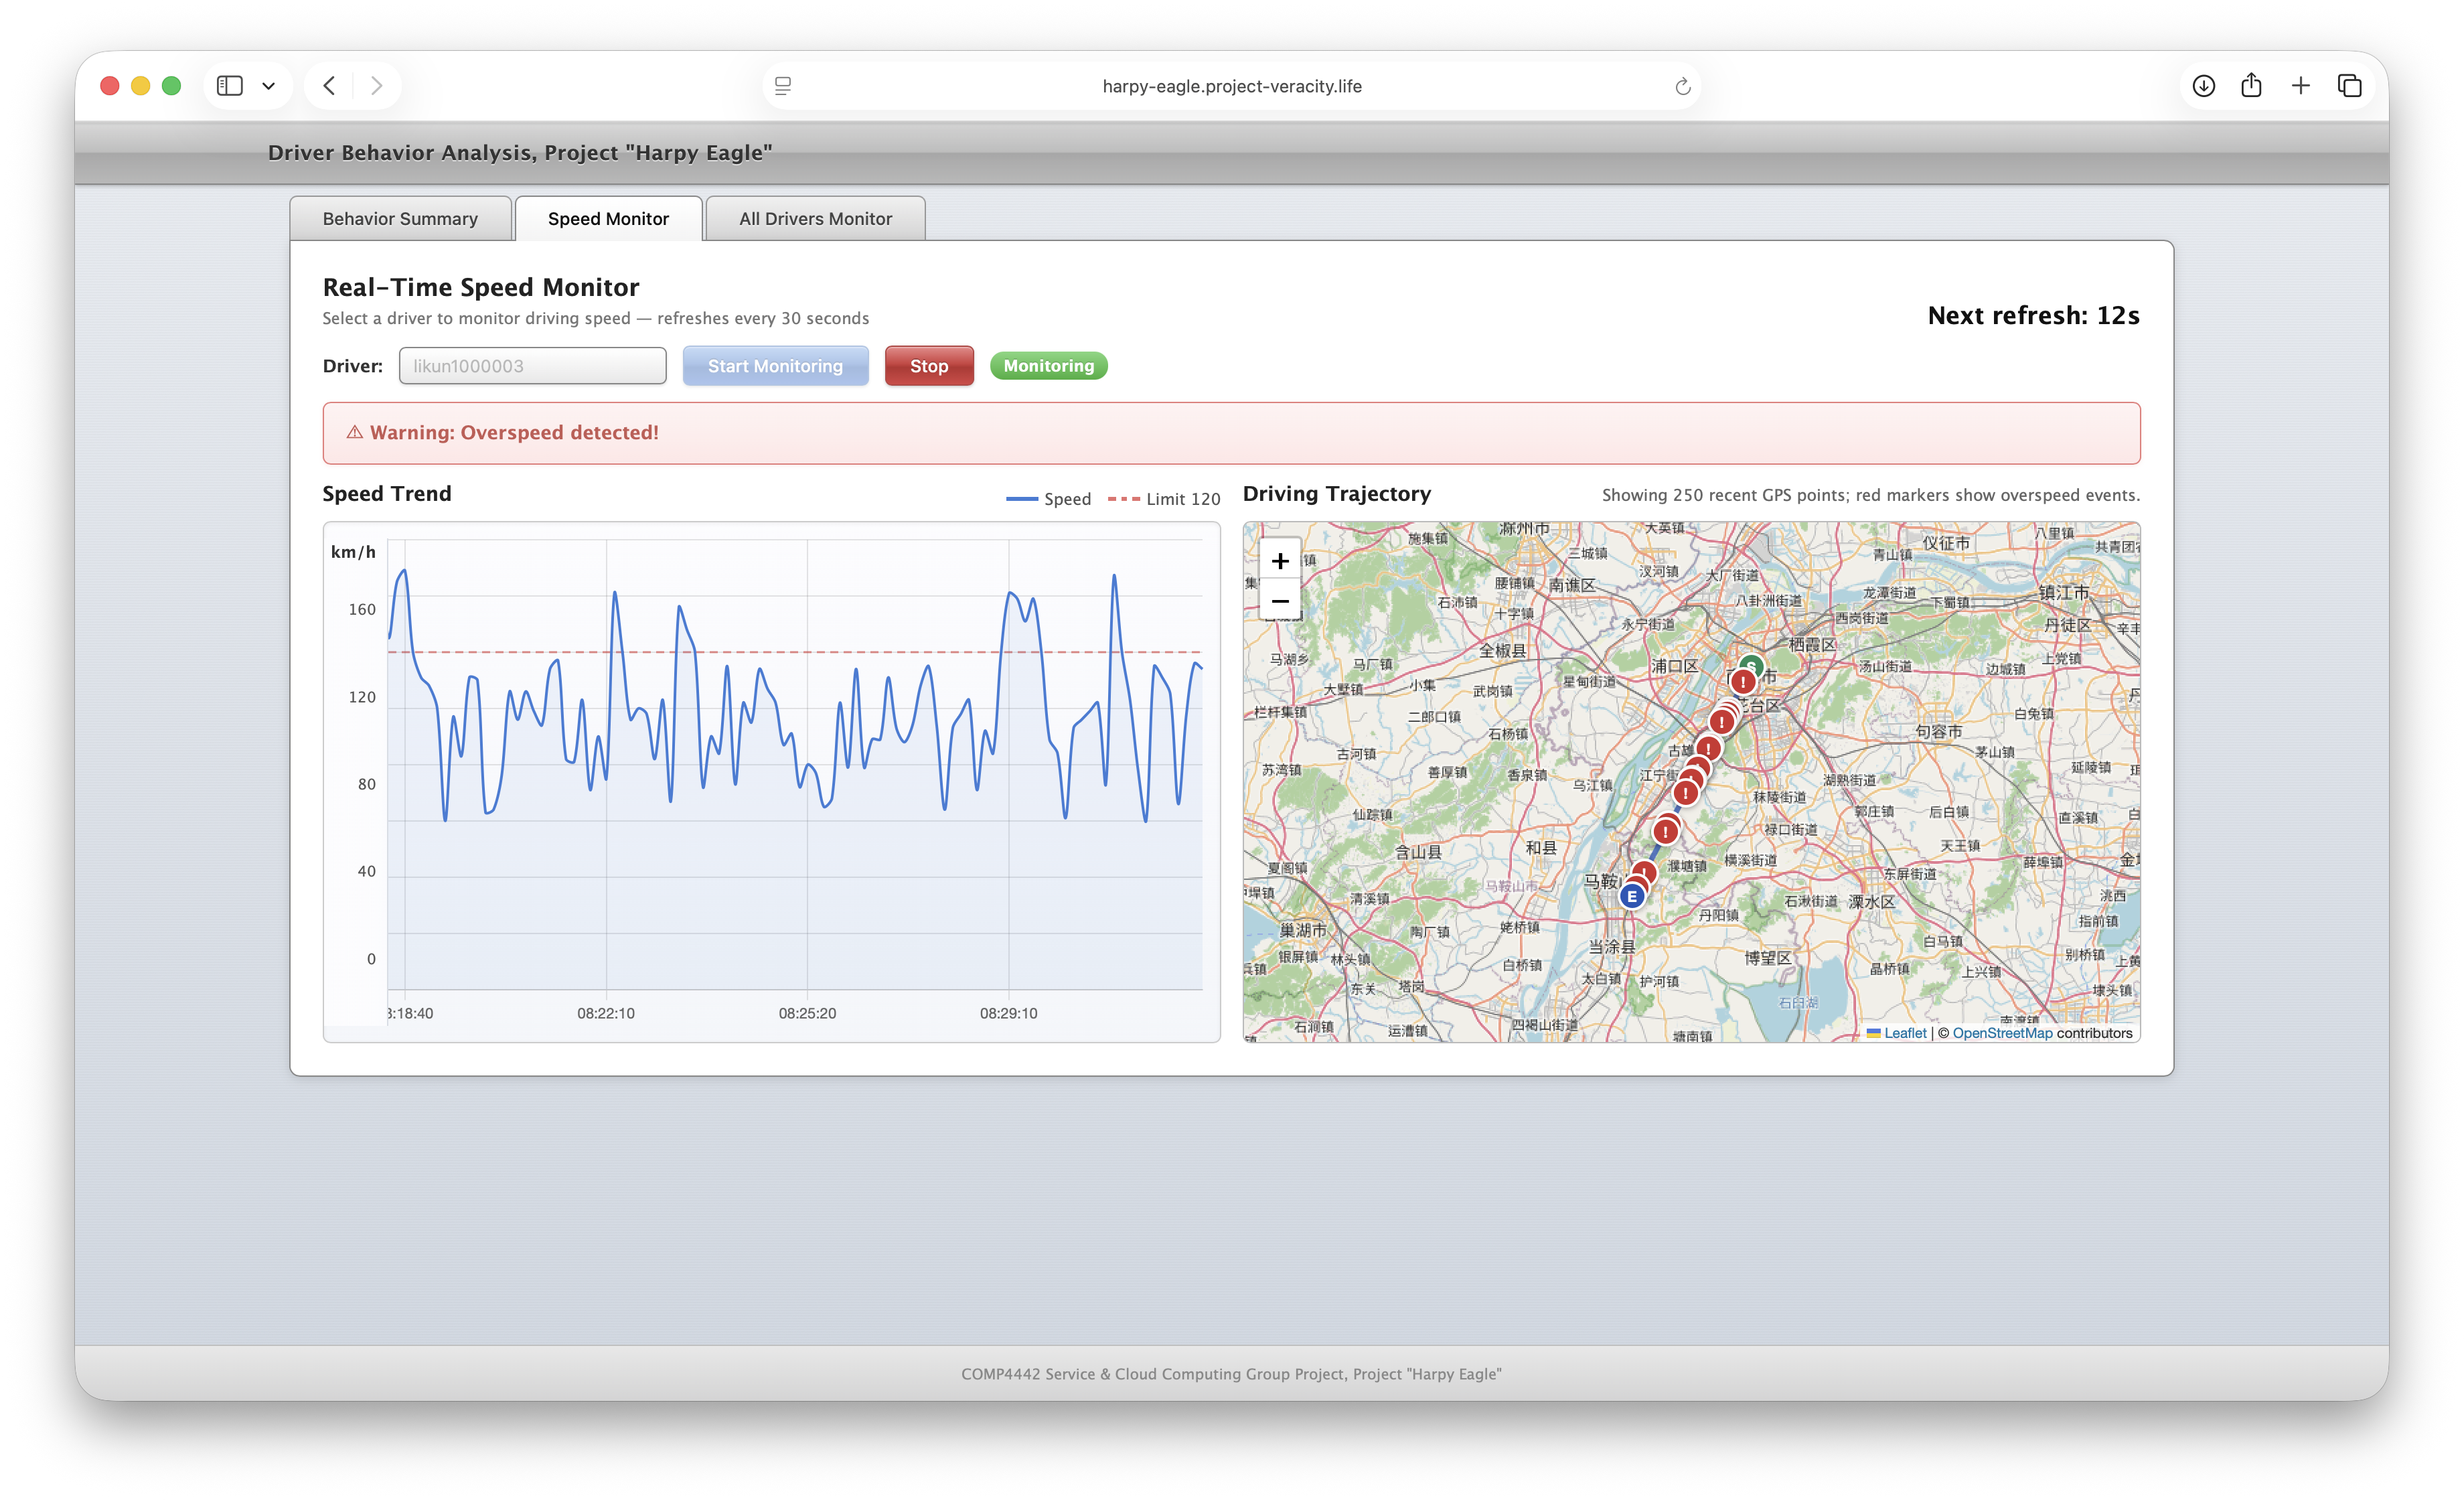
\includegraphics[width=0.9\textwidth]{test-refresh-before.png}
\caption{Speed monitoring before the 30-second refresh}
\label{fig:test-refresh-before}
\end{figure}

\begin{figure}[H]
\centering
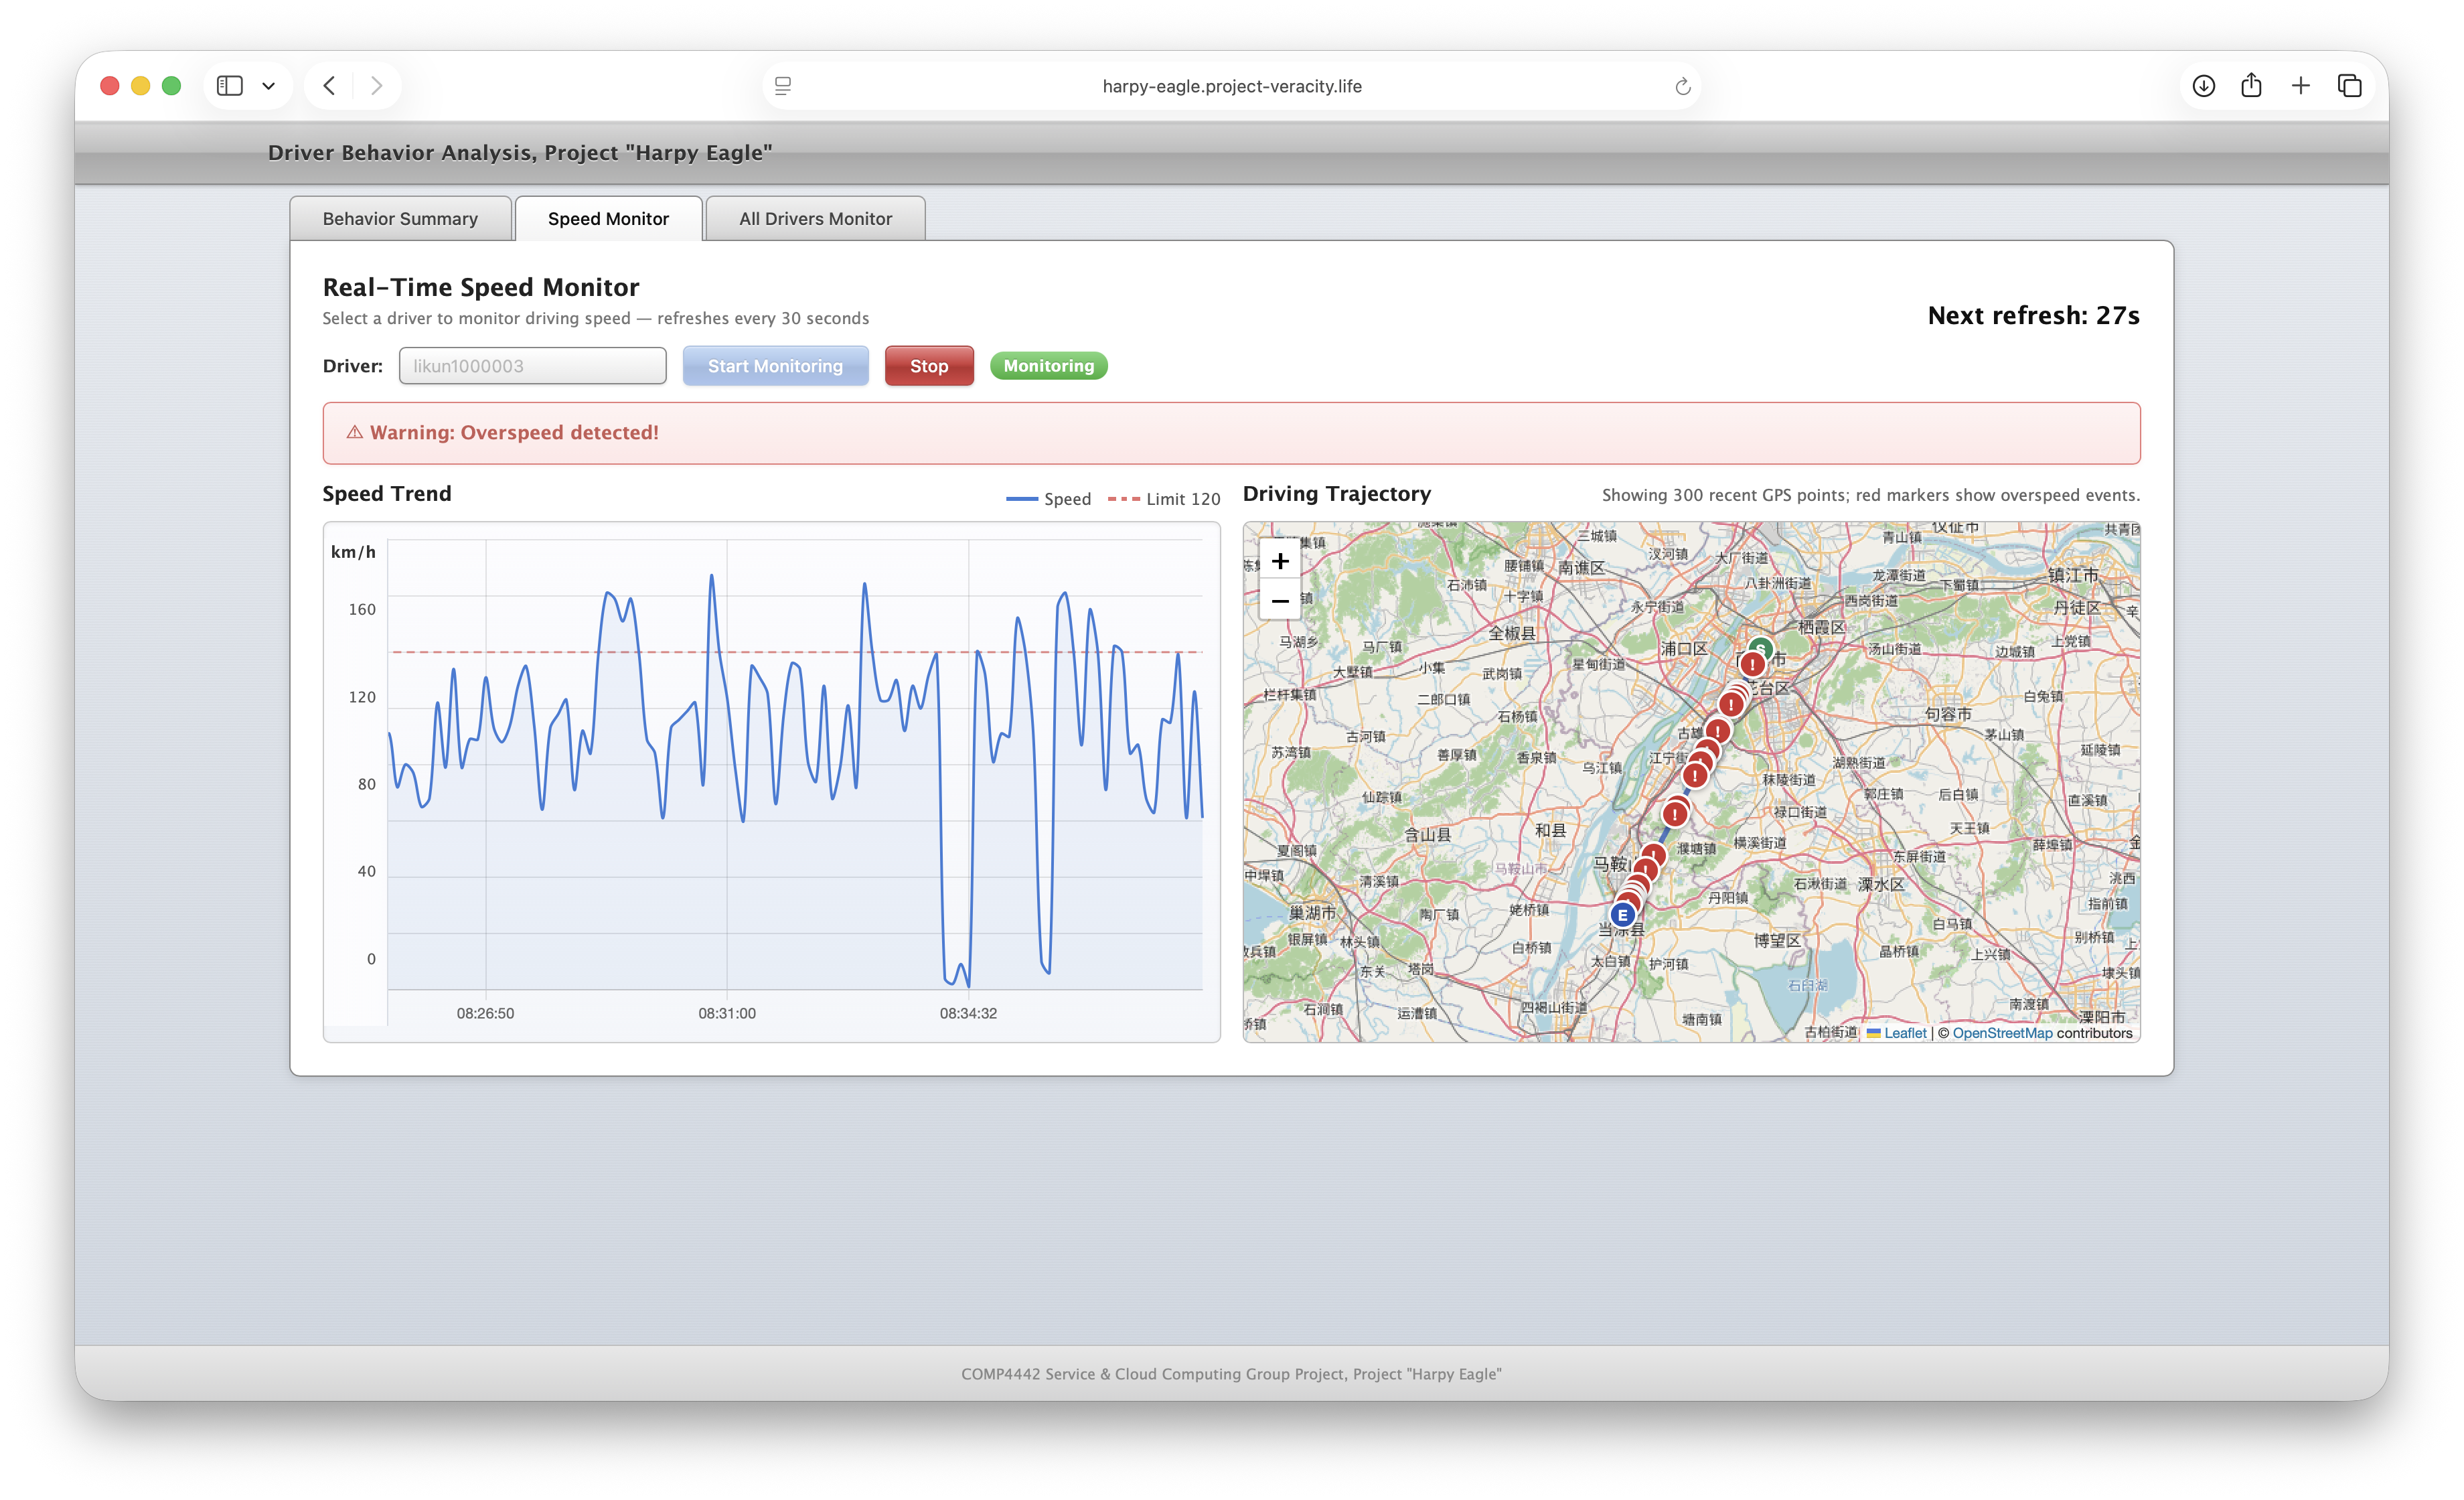
\includegraphics[width=0.9\textwidth]{test-refresh-after.png}
\caption{Speed monitoring after the 30-second refresh}
\label{fig:test-refresh-after}
\end{figure}

\subsubsection{All-Driver Speed Monitoring}

Figure~\ref{fig:test-all-monitor} shows the all-driver monitoring page. The page displays speed curves for all drivers, allowing users to observe the overall speed patterns of the whole dataset.

\begin{figure}[H]
\centering
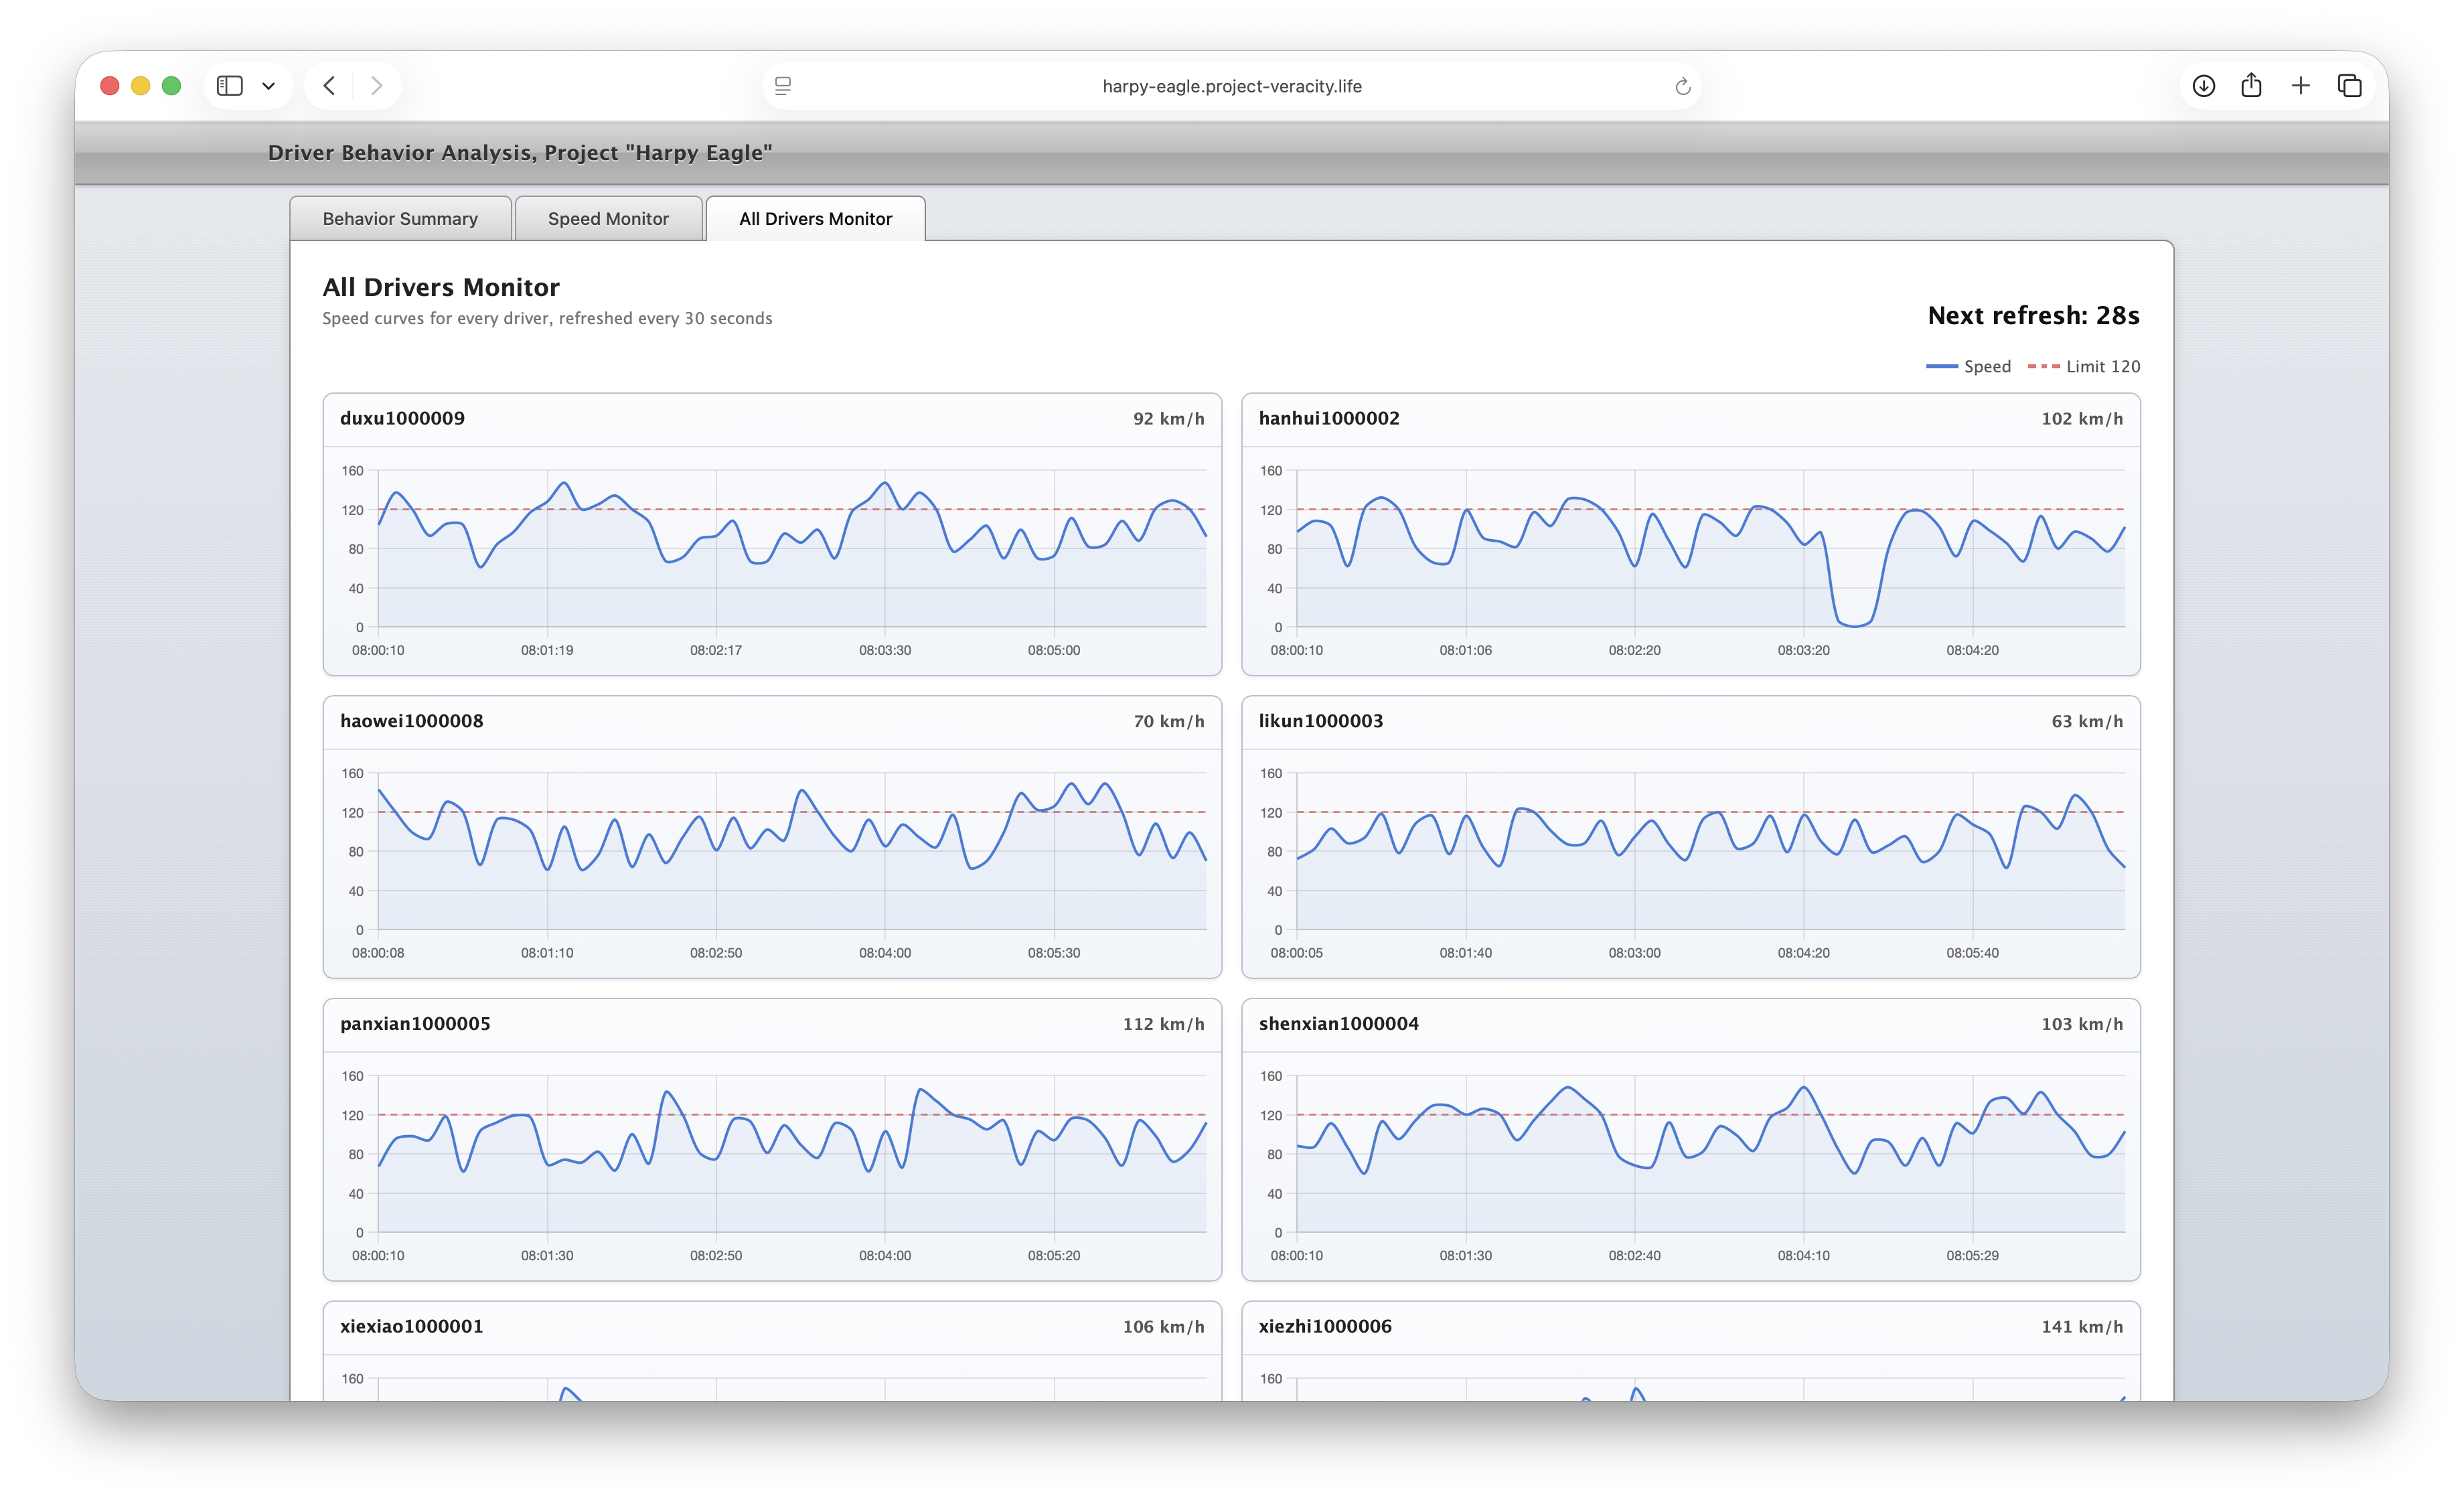
\includegraphics[width=0.9\textwidth]{test-all-monitor.png}
\caption{All-driver speed monitoring test result}
\label{fig:test-all-monitor}
\end{figure}

\subsubsection{Backend API Health Check}

Figure~\ref{fig:test-api-health} shows the backend health check result. The \texttt{/health} and \texttt{/ready} endpoints confirm that the backend service is running and that the DynamoDB-backed dashboard data is configured, accessible, and ready for use.

\begin{figure}[H]
\centering
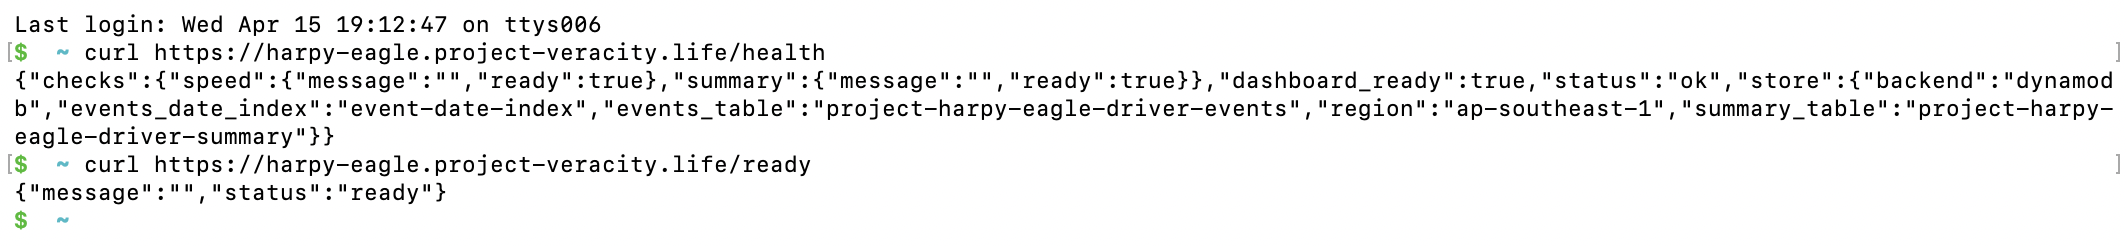
\includegraphics[width=0.9\textwidth]{test-api-health-ready.png}
\caption{Backend health and readiness check result}
\label{fig:test-api-health}
\end{figure}

\subsection{Testing Summary}

The functional testing results show that the system satisfies the main requirements of the project. The website can display driver behavior summaries in a table, calculate and show driver risk rankings, filter behavior statistics by a selected period, monitor the speed of a selected driver, issue overspeed warnings, display the driver's trajectory on a map, and show all drivers' speed curves together. The backend health and readiness checks also confirm that the web service can correctly detect whether the DynamoDB-backed analysis data is available. Therefore, the implemented system is functionally complete for the required driver behavior analysis and real-time speed monitoring tasks.

\section{Summary}

\textit{Harpy Eagle} is a cloud-based driver behavior analysis and real-time monitoring simulation system. The system separates large-scale data processing from online web serving. A PySpark analysis module reads raw driving records from local storage or Amazon S3, applies a fixed schema, and extracts driver IDs, vehicle plates, GPS locations, speed, timestamps, and unsafe-driving indicators. It then writes the processed results directly to Amazon DynamoDB for the web application to query. These results include per-driver behavior summaries, detailed behavior event records for period-based filtering, and per-driver speed time-series data. Based on the processed statistics, the system calculates a normalized driver risk score using weighted factors such as overspeeding, fatigue driving, neutral sliding, rapid acceleration, and rapid deceleration, and classifies each driver into high, medium, or low risk levels.

The Flask backend serves as the bridge between the Spark analytics layer and the frontend dashboard. It reads the processed driver summary, behavior event records, and speed time-series data from Amazon DynamoDB, then exposes REST APIs for driver summaries, available driver lists, batched speed records, and period-based behavior summaries. The backend also includes health and readiness checks to improve deployment reliability.


On the frontend, the dashboard provides three major views: a driver behavior summary page with ranking and datetime period filters, a single-driver speed monitor with Chart.js speed visualization and Leaflet/OpenStreetMap trajectory display, and an all-driver monitoring page for comparing multiple drivers at once.

Overall, in the deployed system, \textbf{Amazon S3} is used to store the raw dataset, Spark script, and EMR logs. \textbf{Amazon EMR} executes the Spark-based batch analysis. The processed driver summary and event records are written directly to \textbf{Amazon DynamoDB}, which is then queried by the Flask web application hosted on \textbf{Amazon EC2} with \textbf{Gunicorn}. We also use \textbf{systemd} to manage the Gunicorn service and \textbf{Cloudflare Tunnel} to provide secure public access without exposing the EC2 application port directly. This architecture combines distributed batch analytics, cloud-managed storage, database-backed RESTful web services, interactive visualization, and secure cloud deployment into an integrated driver safety analysis system.

\end{document}
